    %\ifx\isEmbedded\undefined
%	% Loading common settings
%	\input{macros/common}
%	% Loading common variable definitions 
%	\input{macros/macros}
%	\begin{document} 
%\else
%\fi
%

%\setcounter{chapter}{2}


\chapter{Looking at Images}
\label{chap:looking_at_images}
%\reviewcomment{Unfinished but readable. Text incomplete and missing references.}

\section{Introduction}

Vision is about solving an amazing problem: Can we build a system capable of perceiving its surrounding world using only the information available in the small number of electromagnetic waves that fall into the observer’s sensor (eye or camera), after accidentally bounding off the objects surrounding the observer? How is it possible to sense the world and its three-dimensional (3D) structure without touching it? It seems quite likely that if humans did not have the sense of vision, we would think that solving this problem is impossible. 

The goal of this chapter is to present vision not as an engineering problem that we want to solve, but as a set of scientific questions that we want to answer. We want to understand how it is that our visual system can interpret the world the way it does. We want to explain what components of an image can be used to infer certain properties of the world. We want to know what questions about the world can be answered by just looking at object with the light that reaches our eyes. 

In this chapter we will not answer any of those questions, instead, we will use images to motivate a set of questions that vision scientists and computer vision engineers have been studying for many years. The goal of this chapter is to help you ask questions about how do you perceive the world around you. 

\section{Looking at Individual Pixels}


Before we build systems that can see, it is good to learn to look at images and to pay attention to individual pixels.
\index{Pixel}
The image in \fig{\ref{fig:pexels-retha-ferguson}} is a tiny image with just $32 \times 32$ pixels. 
It is so small that we can actually look at each single pixel and think about how it is that we can make sense of it. For instance, let's look at the pixel in row 21 counting from the top, and column 20 counting from the left. That pixel corresponds to a dark gray pixel, which is near a couple of other pixels with similar intensity, surrounded by a set of white pixels. That pixel seems to be a pen, but how do we know what it is? The pen is barely three pixels long and one pixel wide. How can that provide enough information? 

\begin{figure}[h!]
\centerline{
    %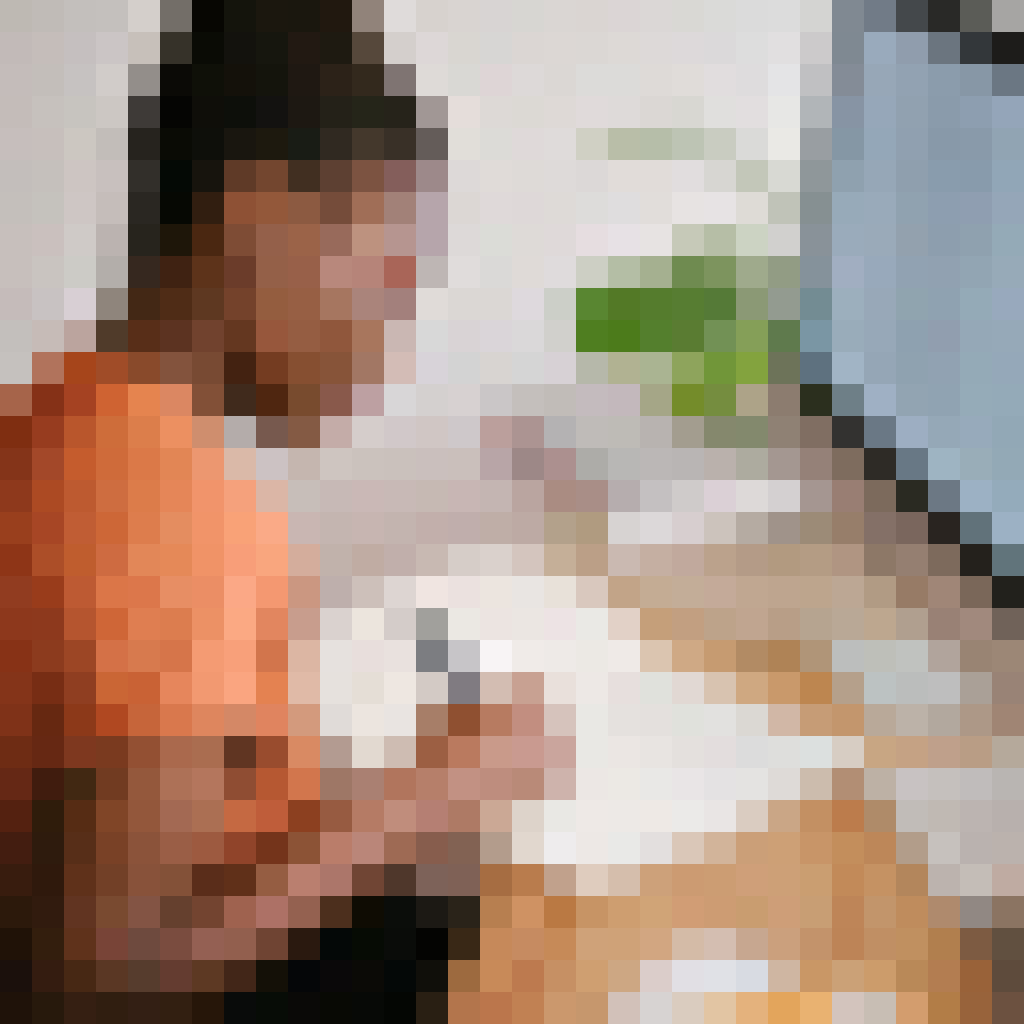
\includegraphics[width=.9\linewidth]{figures/visionscience/pexels-retha-ferguson-3059745_32pixels.jpg}
    
\includegraphics[width=.8\linewidth]{figures/visionscience/DALLE_32x32.png}
    }
    \caption{A tiny image with 32 $\times$ 32 color pixels. Despite the very low resolution, we can still recognize most of its content. {\em Source}: Original image created with Dall-E, and downsampled with Photoshop.}
    \label{fig:pexels-retha-ferguson}
\end{figure}
% Finally not used: Photo by Retha Ferguson from Pexels
% Original: https://www.pexels.com/photo/woman-in-front-of-her-computer-3059745/
% https://markallenassets.blob.core.windows.net/communitycare/2020/11/edit.Retha-Ferguson-from-Pexels-woman-in-front-of-her-computer-3059745.png
% we use instead photo generated with Dall-E


\marginnote{
Same image as in \fig{\ref{fig:pexels-retha-ferguson}} but shown small. 
\\[6pt]
\centerline{

\includegraphics[width=.20\linewidth]{figures/visionscience/DALLE_32x32.png}}
\\[6pt]
Reducing the size helps better recognizing the objects despite containing the same visual information. 
}[-3in]

Recognition of the meaning of that pixel can not come just from the intensity of that pixel or the few pixels nearby. There are way too many possible situations in which different objects in the world could map to a similar set of pixel intensities. Instead, is the whole image and the context of the pen that provides the necessary information to recognize the pen. Taken in isolation, those pixels are impossible to recognize. Here we show, from left to right, the hand, the pen, and the blue mug.


\begin{figure}[h!]
\centerline{
    
\includegraphics[width=.17\linewidth]{figures/visionscience/dalle_hand.png}
    ~
    
\includegraphics[width=.34\linewidth]{figures/visionscience/dalle_mug.png}
    ~
    
\includegraphics[width=.29\linewidth]{figures/visionscience/dalle_pen.png}
    %~
    %
\includegraphics[width=.21\linewidth]{figures/visionscience/plant.png}
    }
    \caption{Small image patches from \fig{\ref{fig:pexels-retha-ferguson}} in isolation. It is difficult to recognize image patches outside their natural context.}
    %\label{fig:image_classification}
\end{figure}

%\centerline{
%
\includegraphics[width=.15\linewidth]{figures/visionscience/pexels-retha-ferguson-3059745_32blur.jpg}
%}


\marginnote{What is the minimum number of pixels needed to form a recognizable image? The answer depends on the image. It is possible to create visually recognizable images with very few pixels \cite{torralba_2009}.}


\section{The More You Look, the More You See}
%{\bf The more you look, the more you see.} 
Visual perception cannot be formulated as a simple input-output function over predefined domains. Vision is a dynamical system, even when looking at a static image. The longer you look at an image, the more details you see and the better you understand the scene. Just look at the image shown in \fig{\ref{fig:street_in_paris}} and try to write down everything you see down to the smallest detail. 

% Some useful reference: https://www.pnas.org/content/112/12/3618

% http://groups.csail.mit.edu/vision/datasets/ADE20K//ADE20K_2016_07_26/images/training/r/restaurant_patio/ADE_train_00015819.jpg
\begin{figure}[t]
\centerline{
    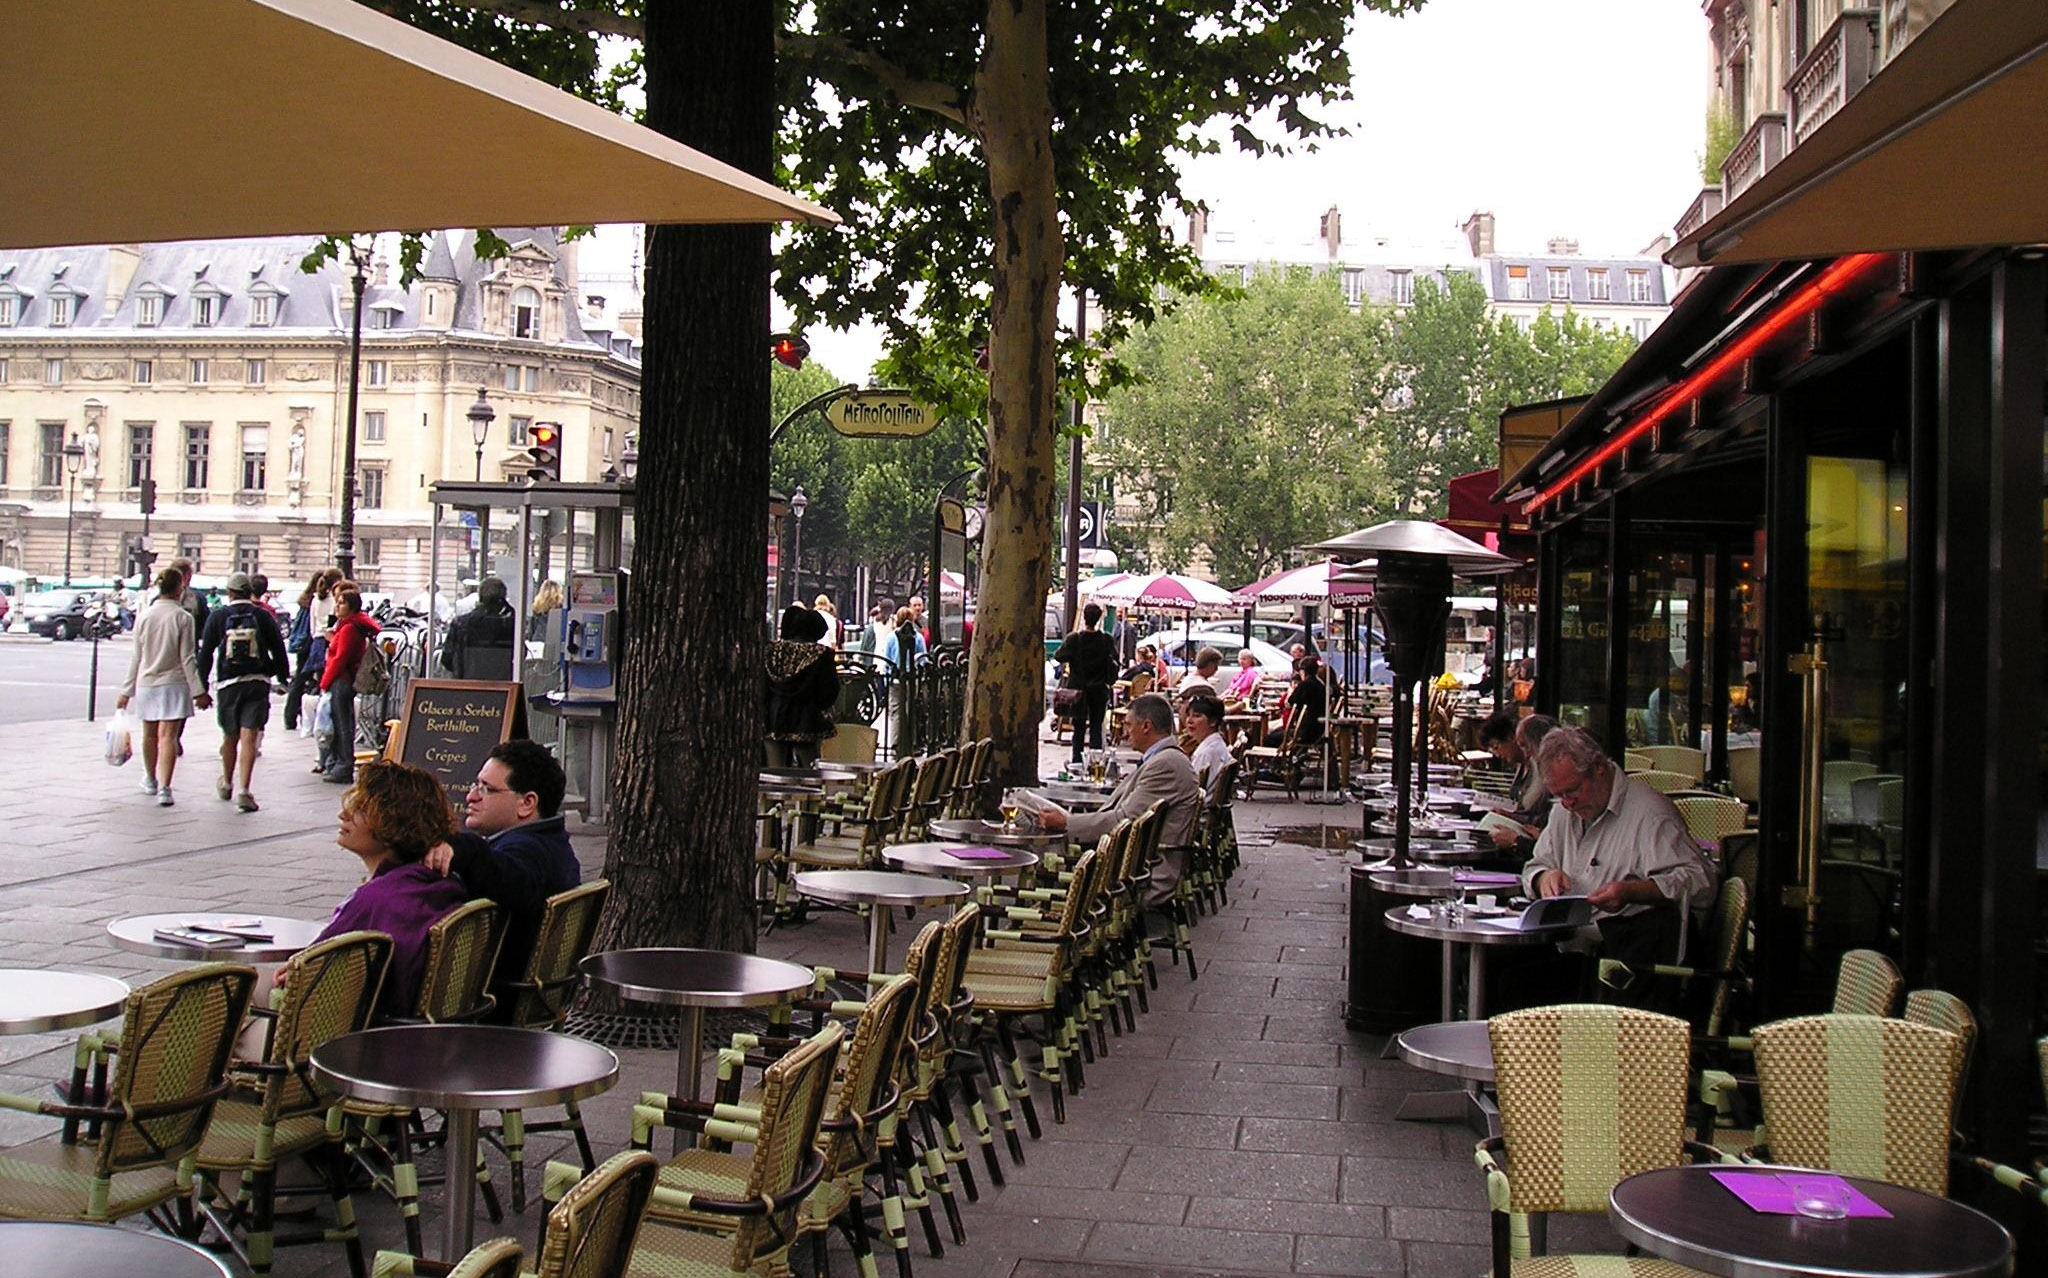
\includegraphics[width=.98\linewidth]{figures/visionscience/ADE_train_00015819_messed_small.jpg}
    }
    \caption{A street in Paris. Is everything fine in this picture?}
    \label{fig:street_in_paris}
\end{figure}
% Photo by Antonio Torralba


But this feeling of unlimited and effortless understanding of a picture is also an illusion. Do you truly understand everything you see? For instance, are you sure you can make sense of all the chair legs in \fig{\ref{fig:street_in_paris}}? In fact, this image has been manipulated so that some of legs do not correspond to any chair.

\marginnote{When solving a task, as the {\bf visual cognitive load} increases we are more likely to make judgment mistakes.
% https://graphics.stanford.edu/papers/visual-cognitive-load/klingner_aural_vs_visual_cognitive_load.pdf
}

As you look around the image, notice that each patch you look at is actually a small photo in its own right. In fact, a big image like this contains thousands of tiny images within it (\fig{\ref{fig:tiny_images}}). A single photo can be \textit{big data}; if you chop up this photo you get a big dataset of tiny images.
A common trick in computer vision is to take a method that was developed for processing a dataset and instead apply it to the set of patches in an image, or vice versa.


\begin{figure}[t]
\centerline{
    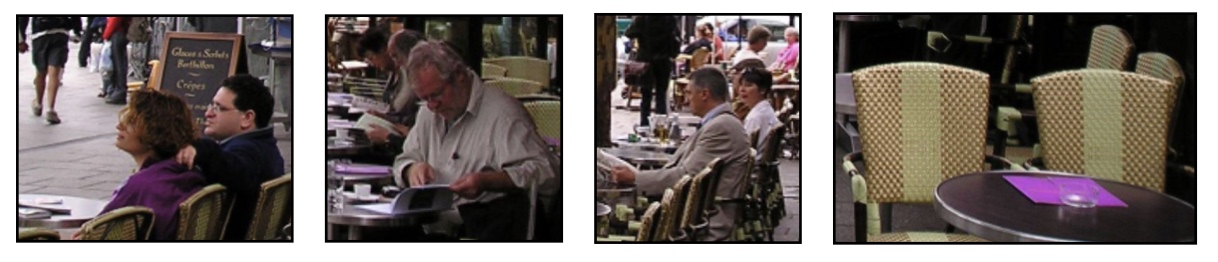
\includegraphics[width=1\linewidth]{figures/visionscience/tiny_images.jpg}
    }
    \caption{Each picture contains lots of images.}
    \label{fig:tiny_images}
\end{figure}


% \begin{center}
%     patch : image :: image : dataset
% \end{center}

\section{The Eye of the Artist}

Learning to paint is a great way of learning to see. You start from a white piece of canvas and a finite set of acrylic paints, and your goal is to paint an object that should look real, with shadows, 3D shape, and reflections. What mixtures of paint and what strokes can accomplish that? Artists learn to see the world not by what it represents, but as why it looks the way it does. 

The following sequence (\fig{\ref{fig:agata_painting}}), painted by Agata Lapedriza, shows different steps in the painting process of a strawberry. Layer after layer, the artist replicates the light that will fool your eye into seeing a strawberry instead of acrylic paint. It is interesting to see that the realism does not increase monotonically as the painting progresses. For instance, from step 3 to 4, the right side of the strawberry has lost realism. However, those new strokes will become the shading that will make the strawberry pop out from the canvas. 

\begin{figure}
\centerline{
    ~1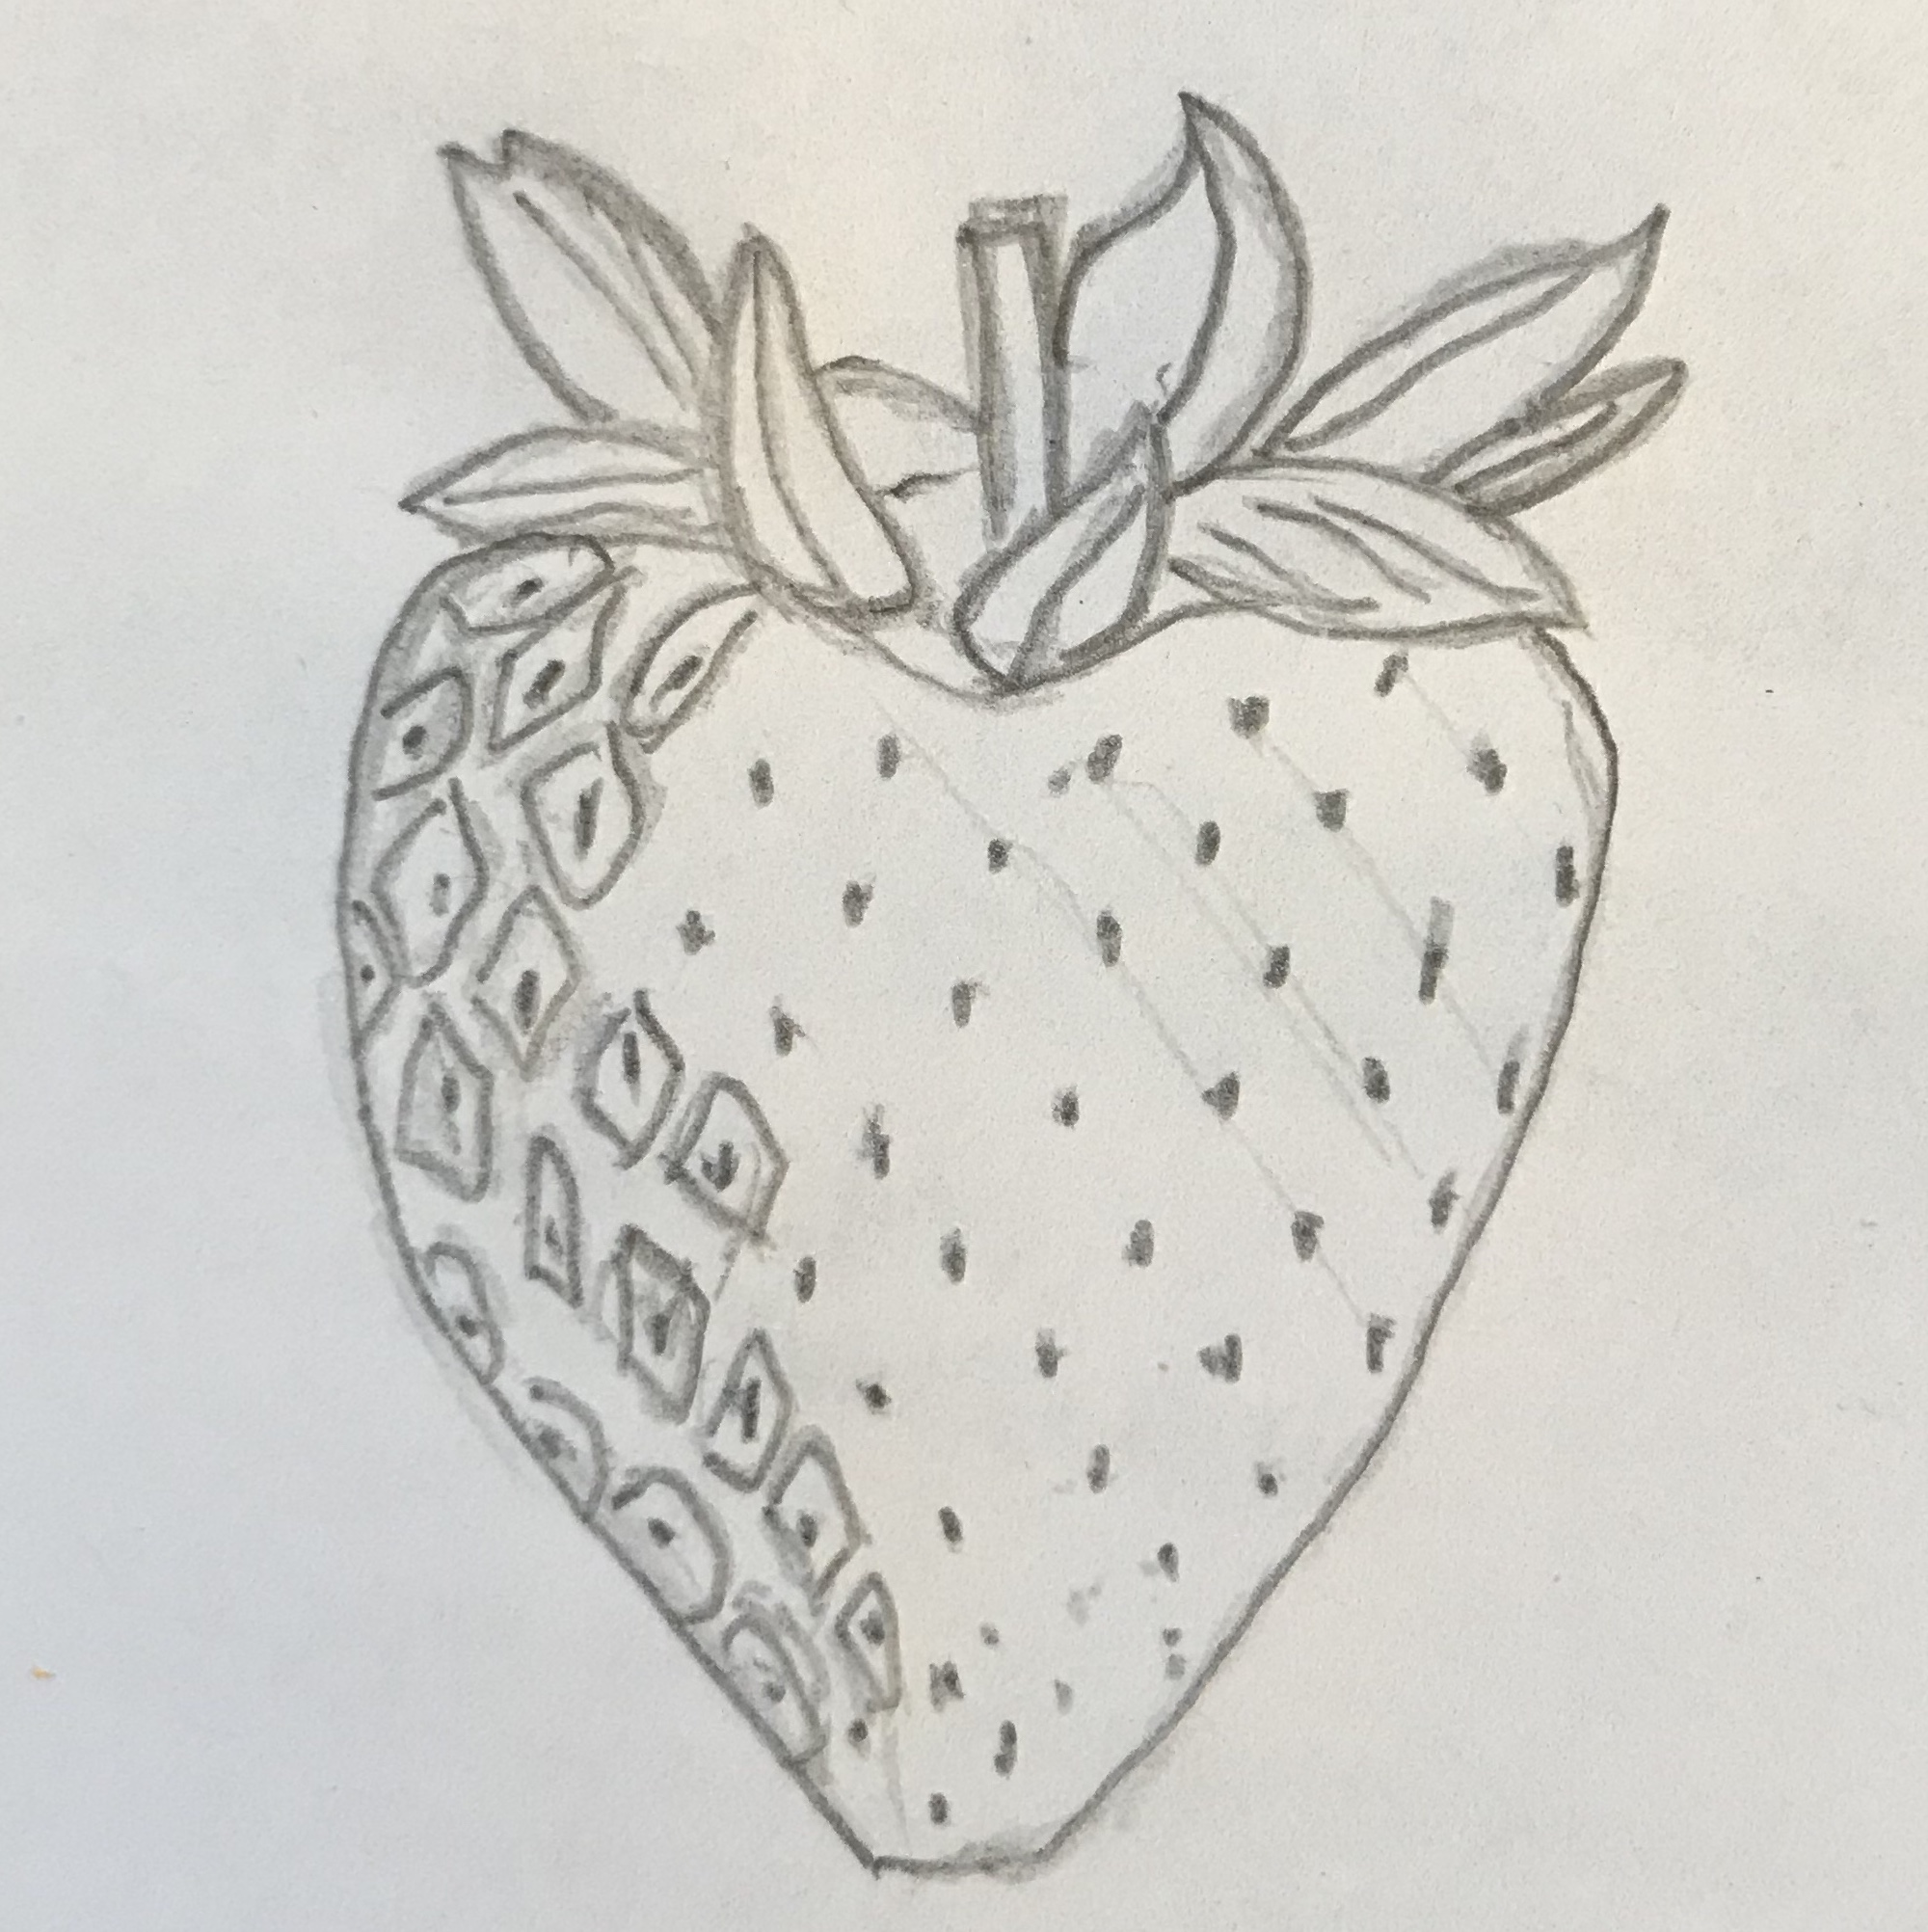
\includegraphics[width=.22\linewidth]{figures/visionscience/fresa_1.jpg}
    2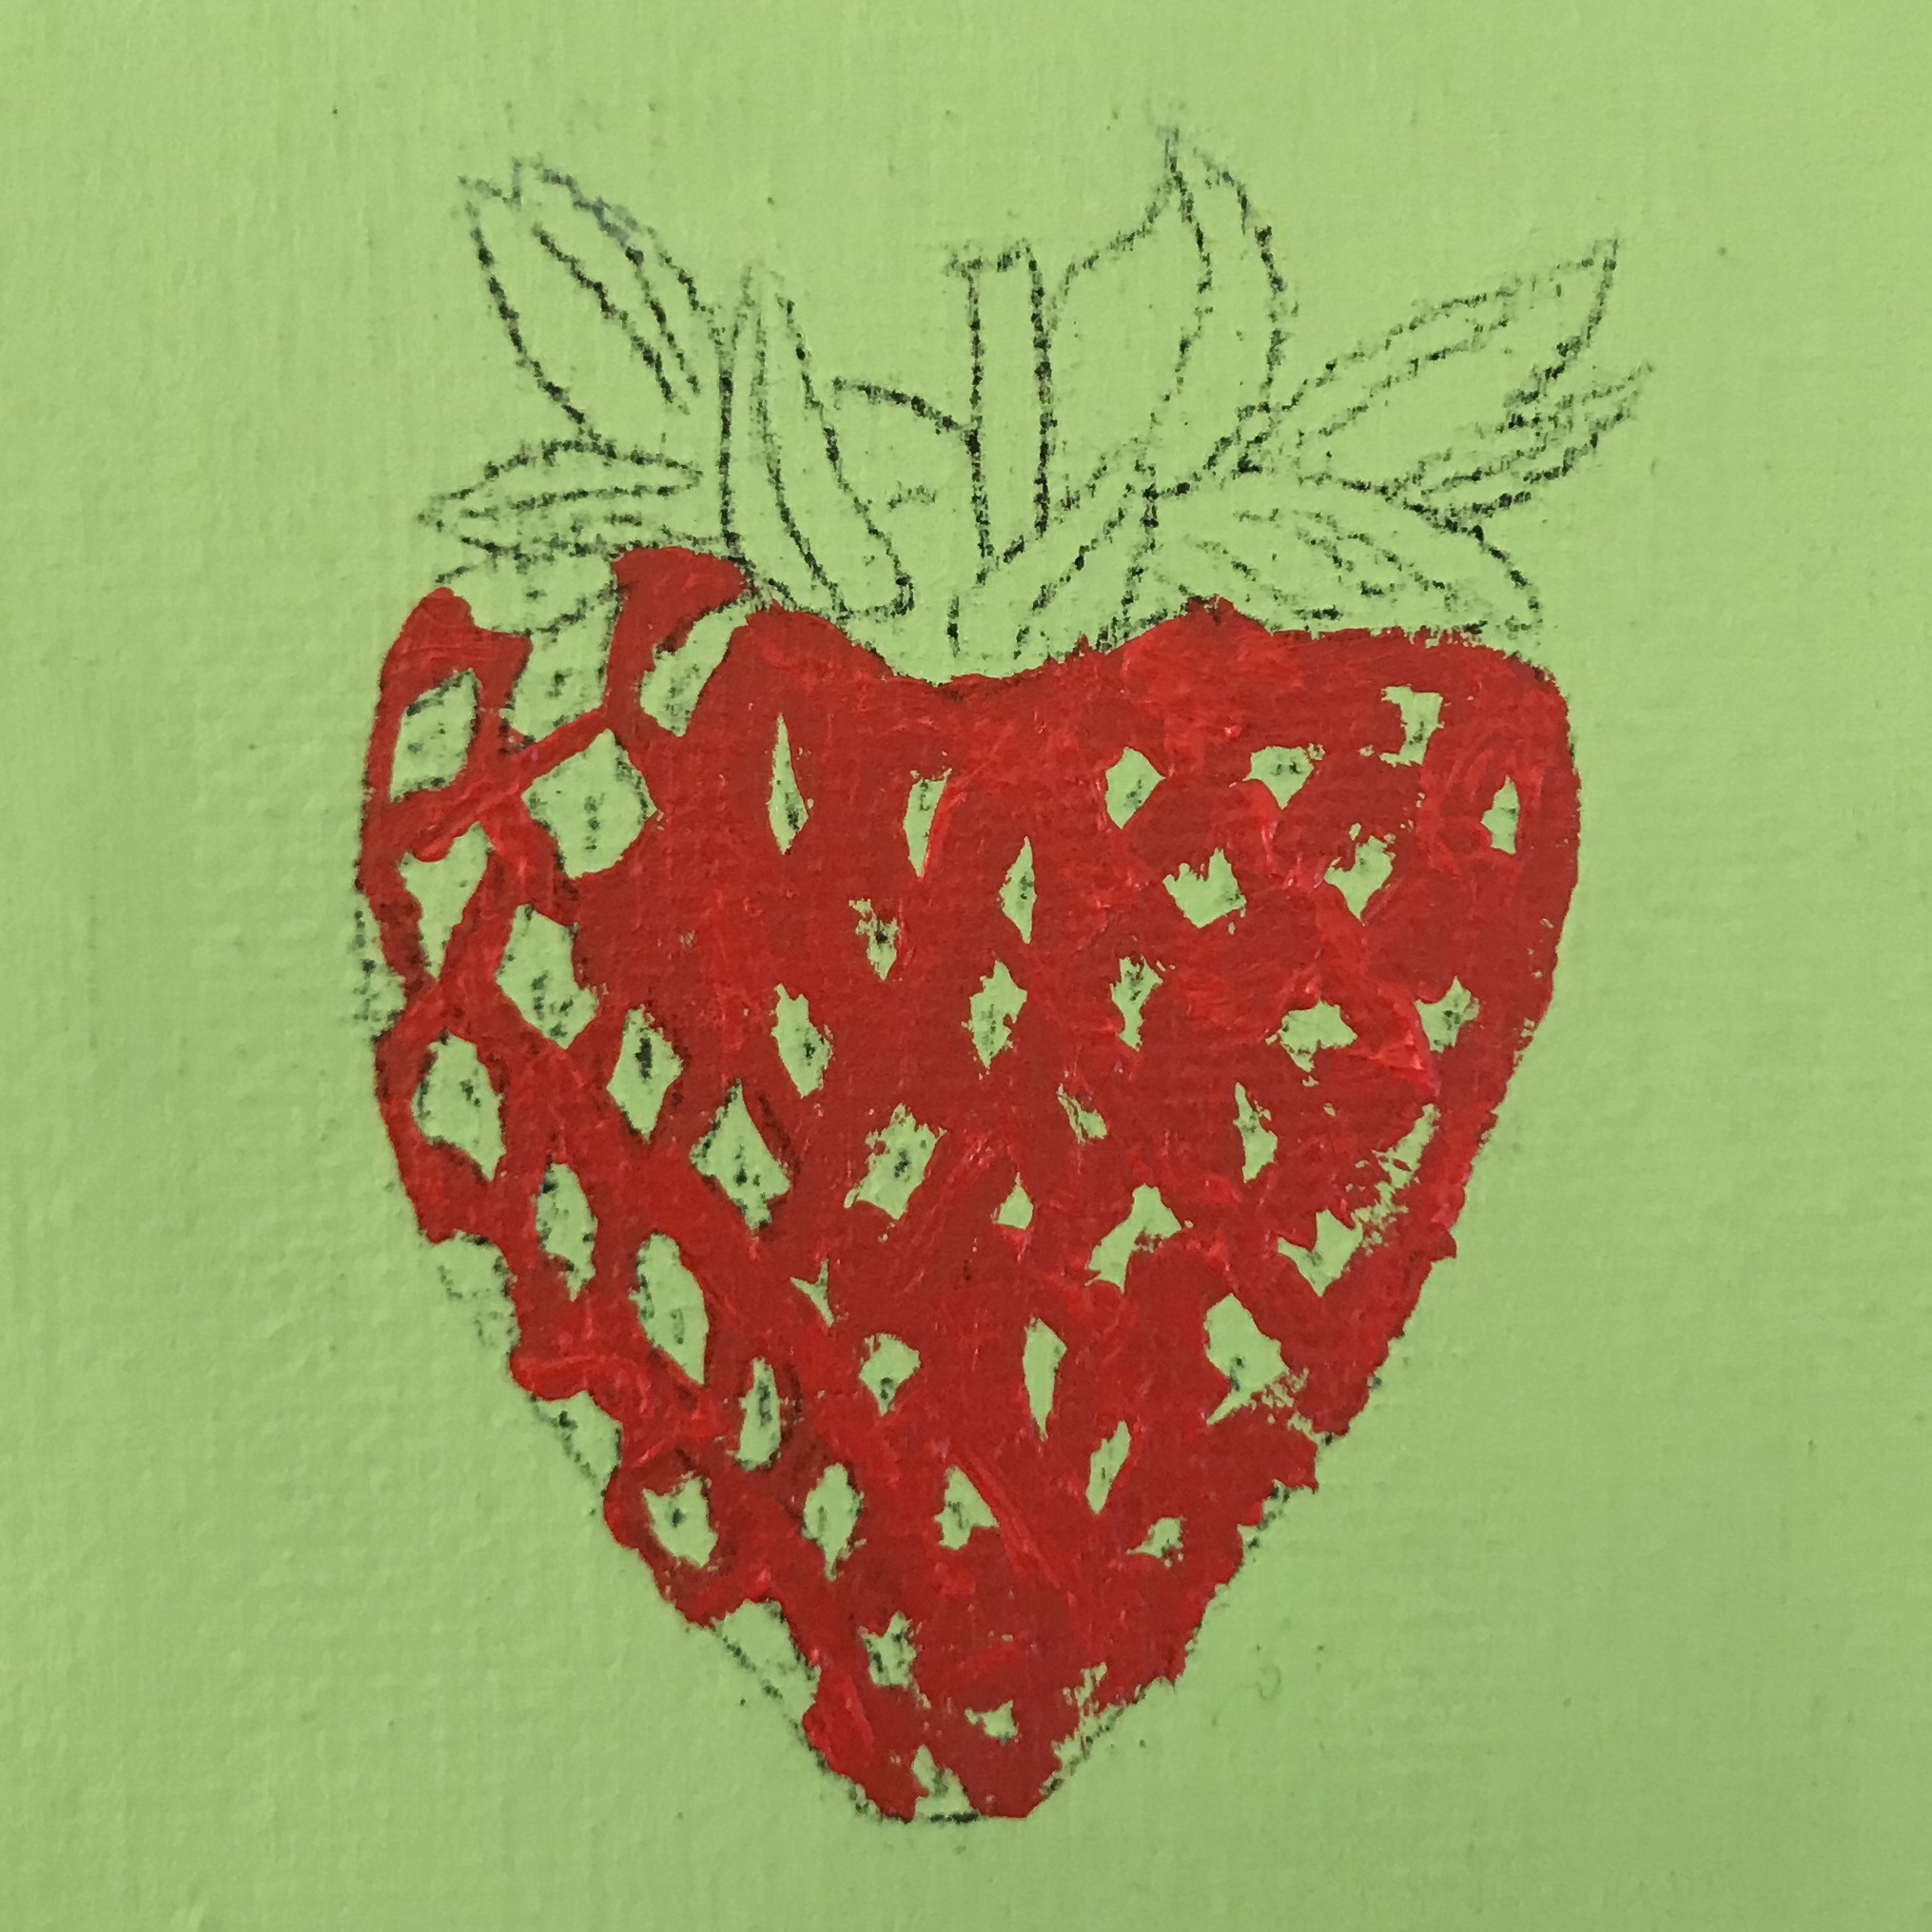
\includegraphics[width=.22\linewidth]{figures/visionscience/fresa_2.jpg}
    3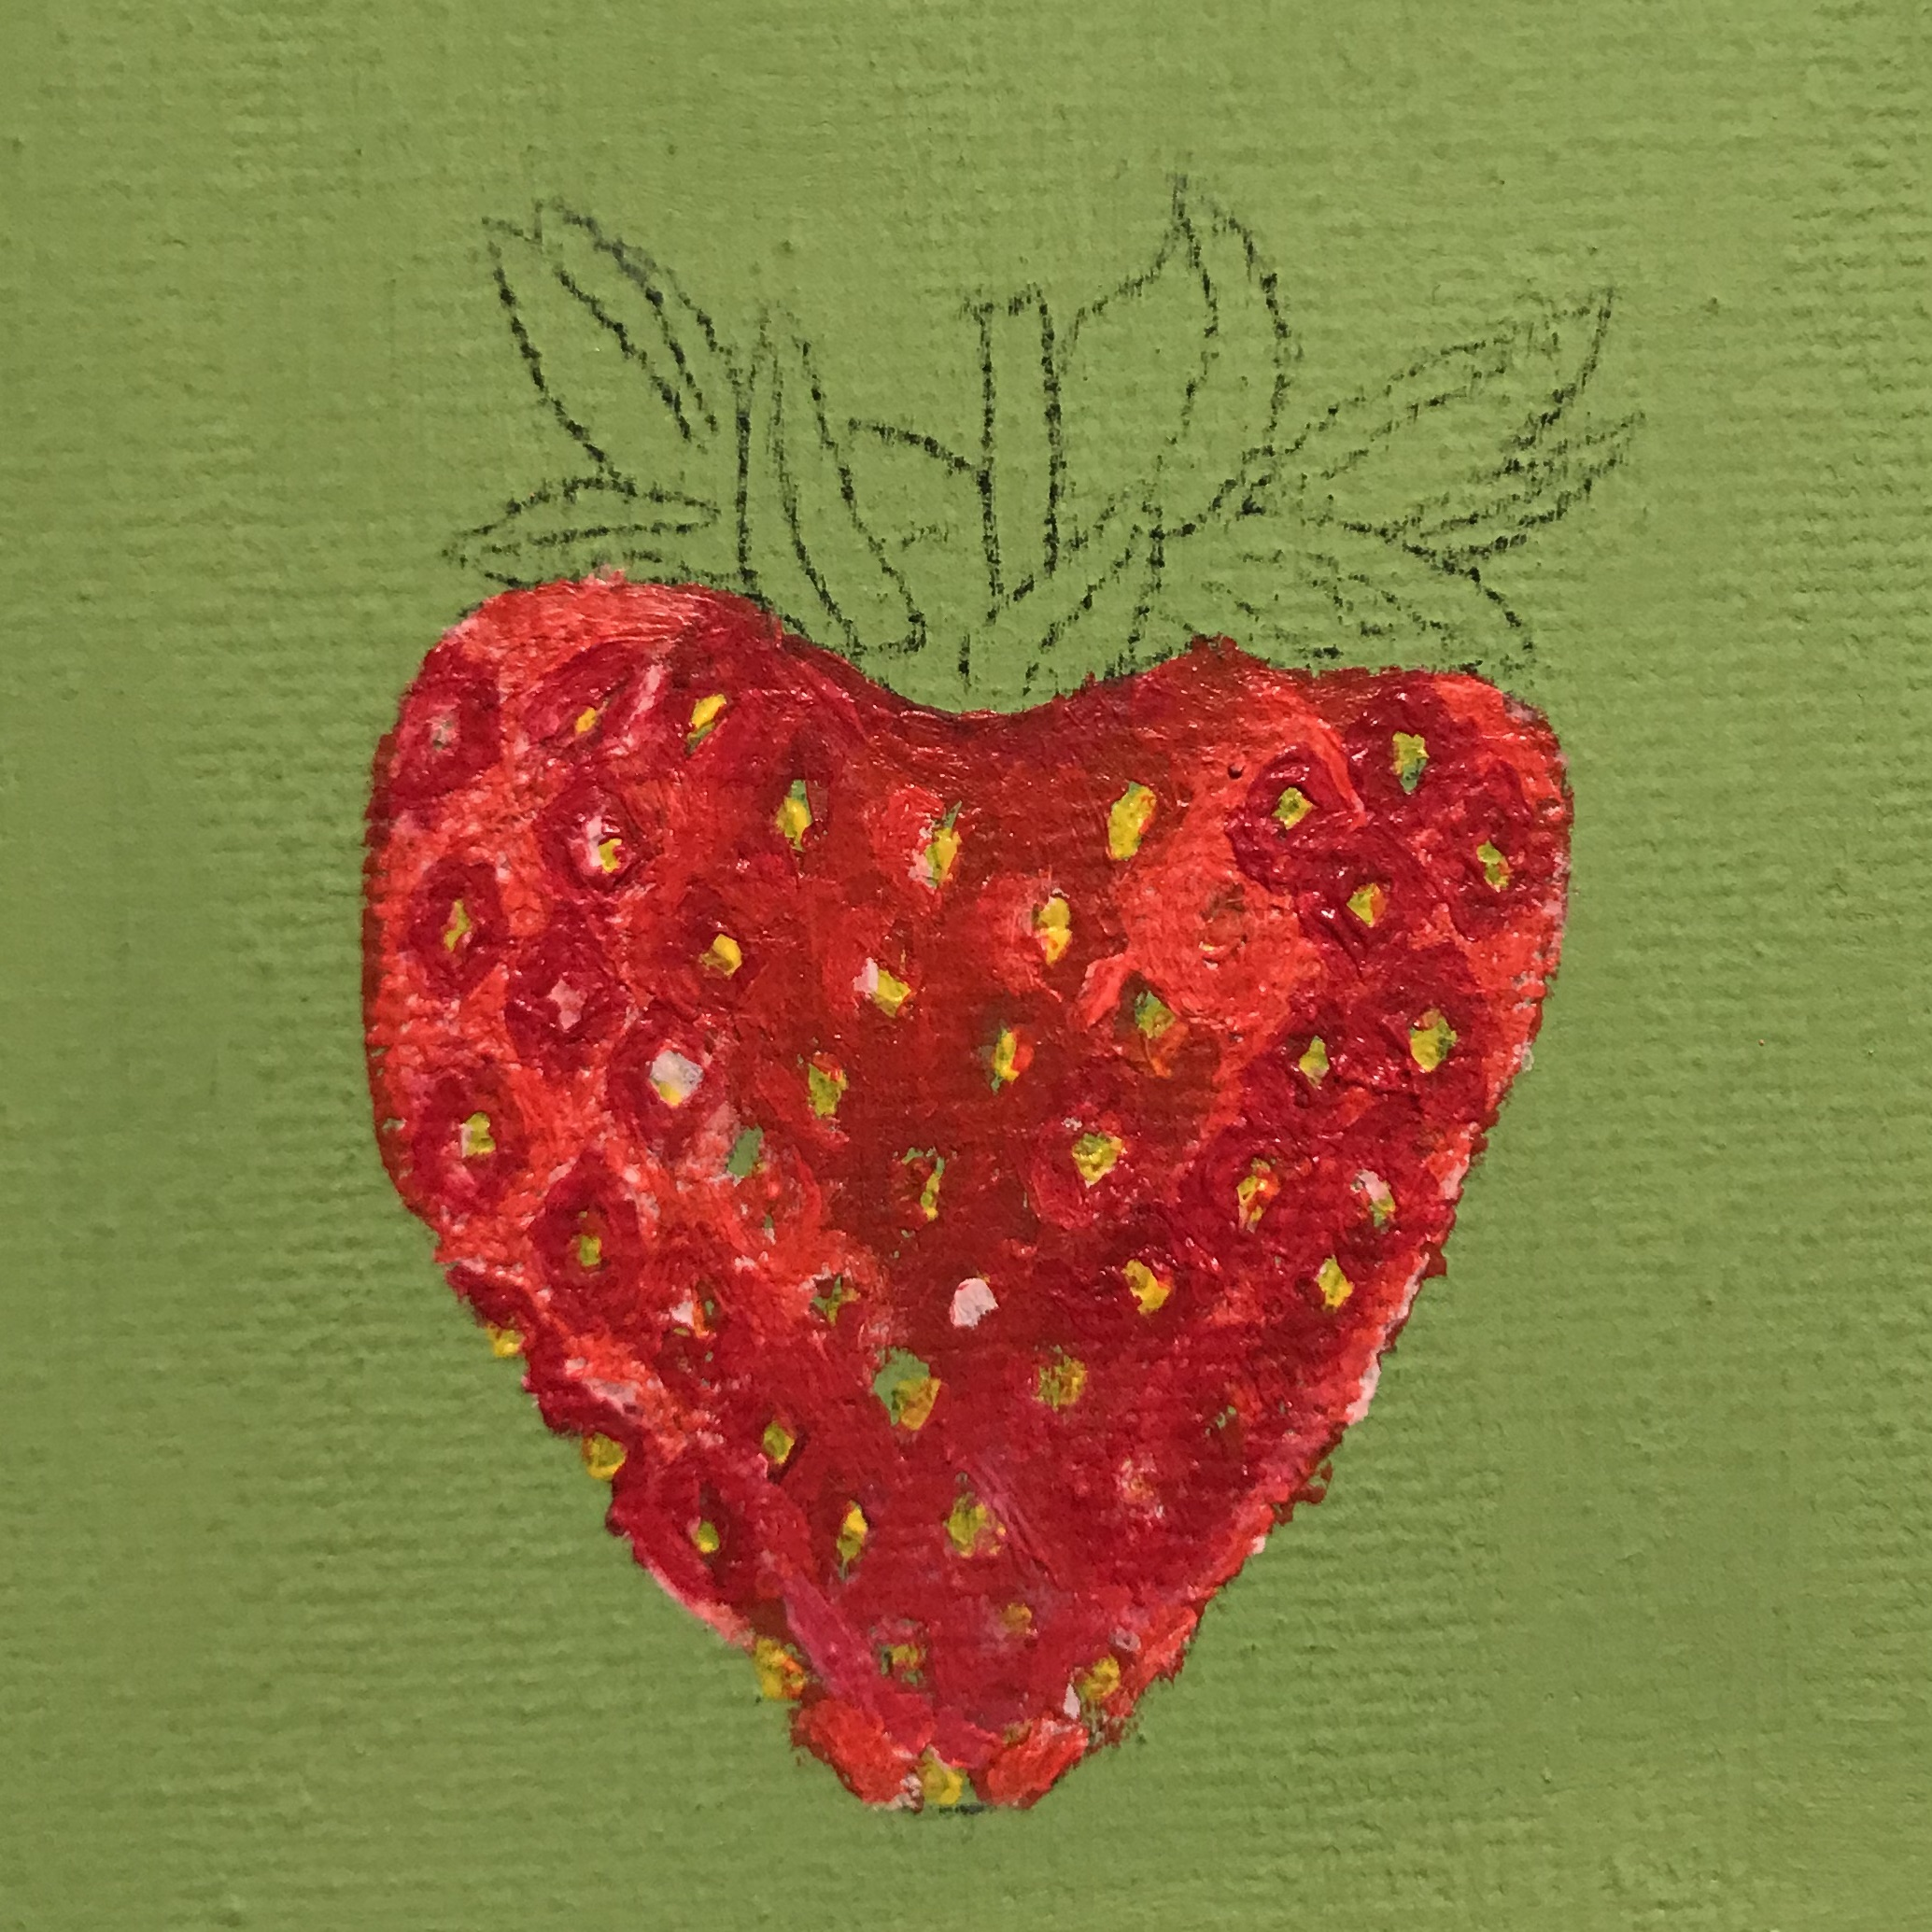
\includegraphics[width=.22\linewidth]{figures/visionscience/fresa_3.jpg}
    4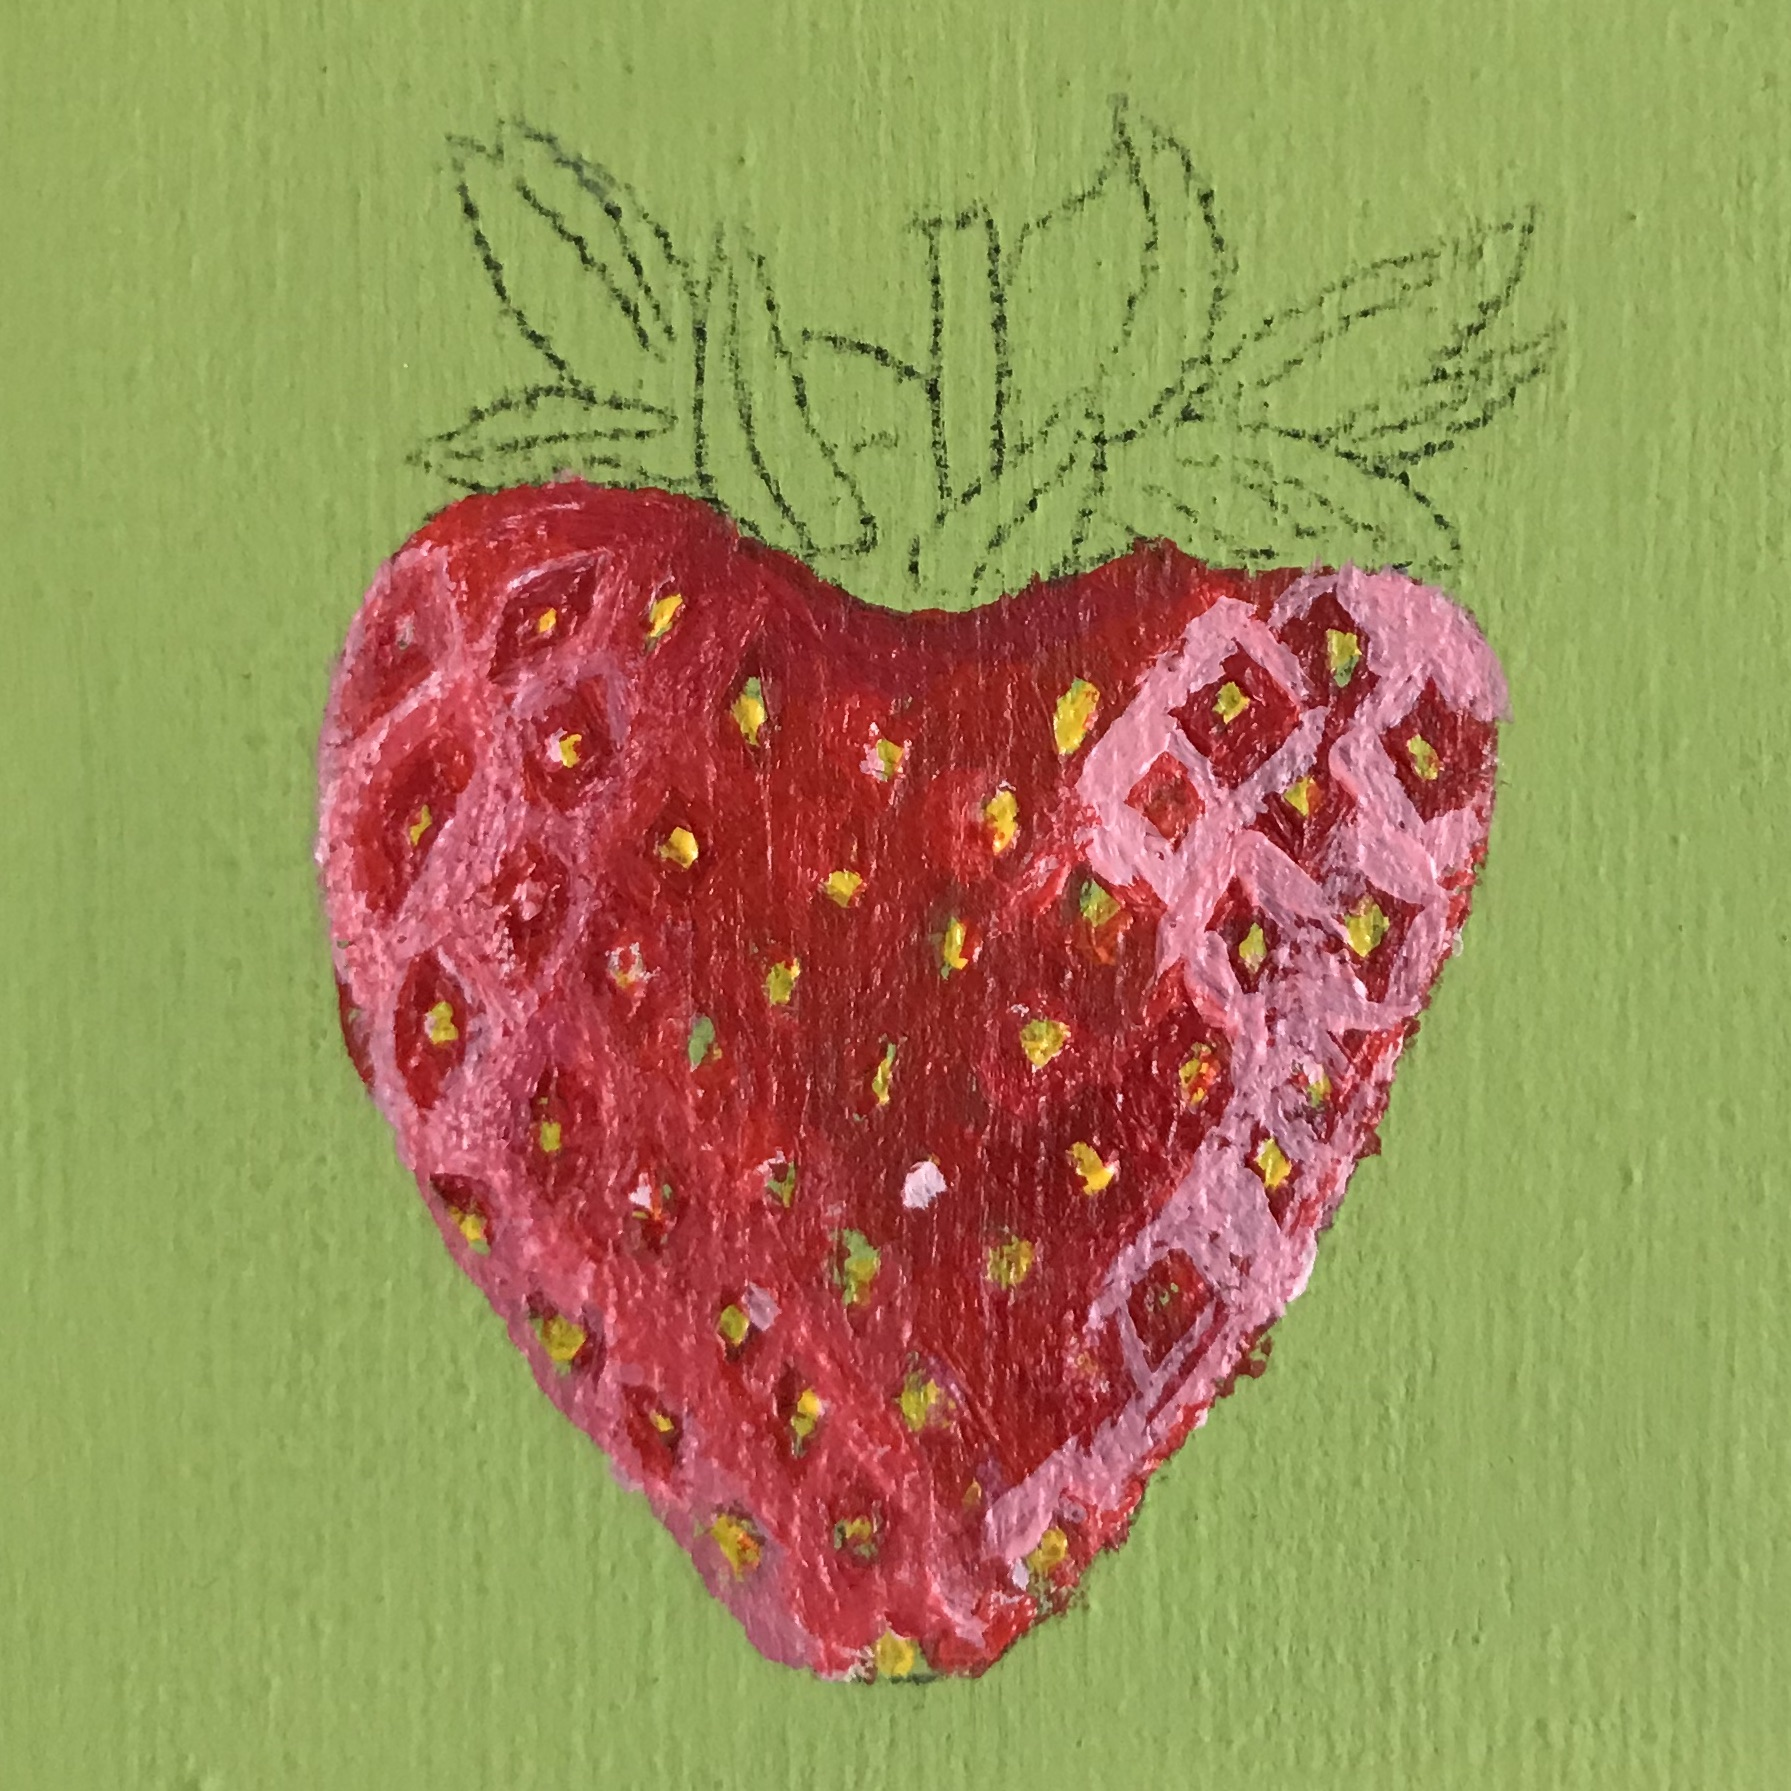
\includegraphics[width=.22\linewidth]{figures/visionscience/fresa_4.jpg}
    }
    \centerline{
    ~~5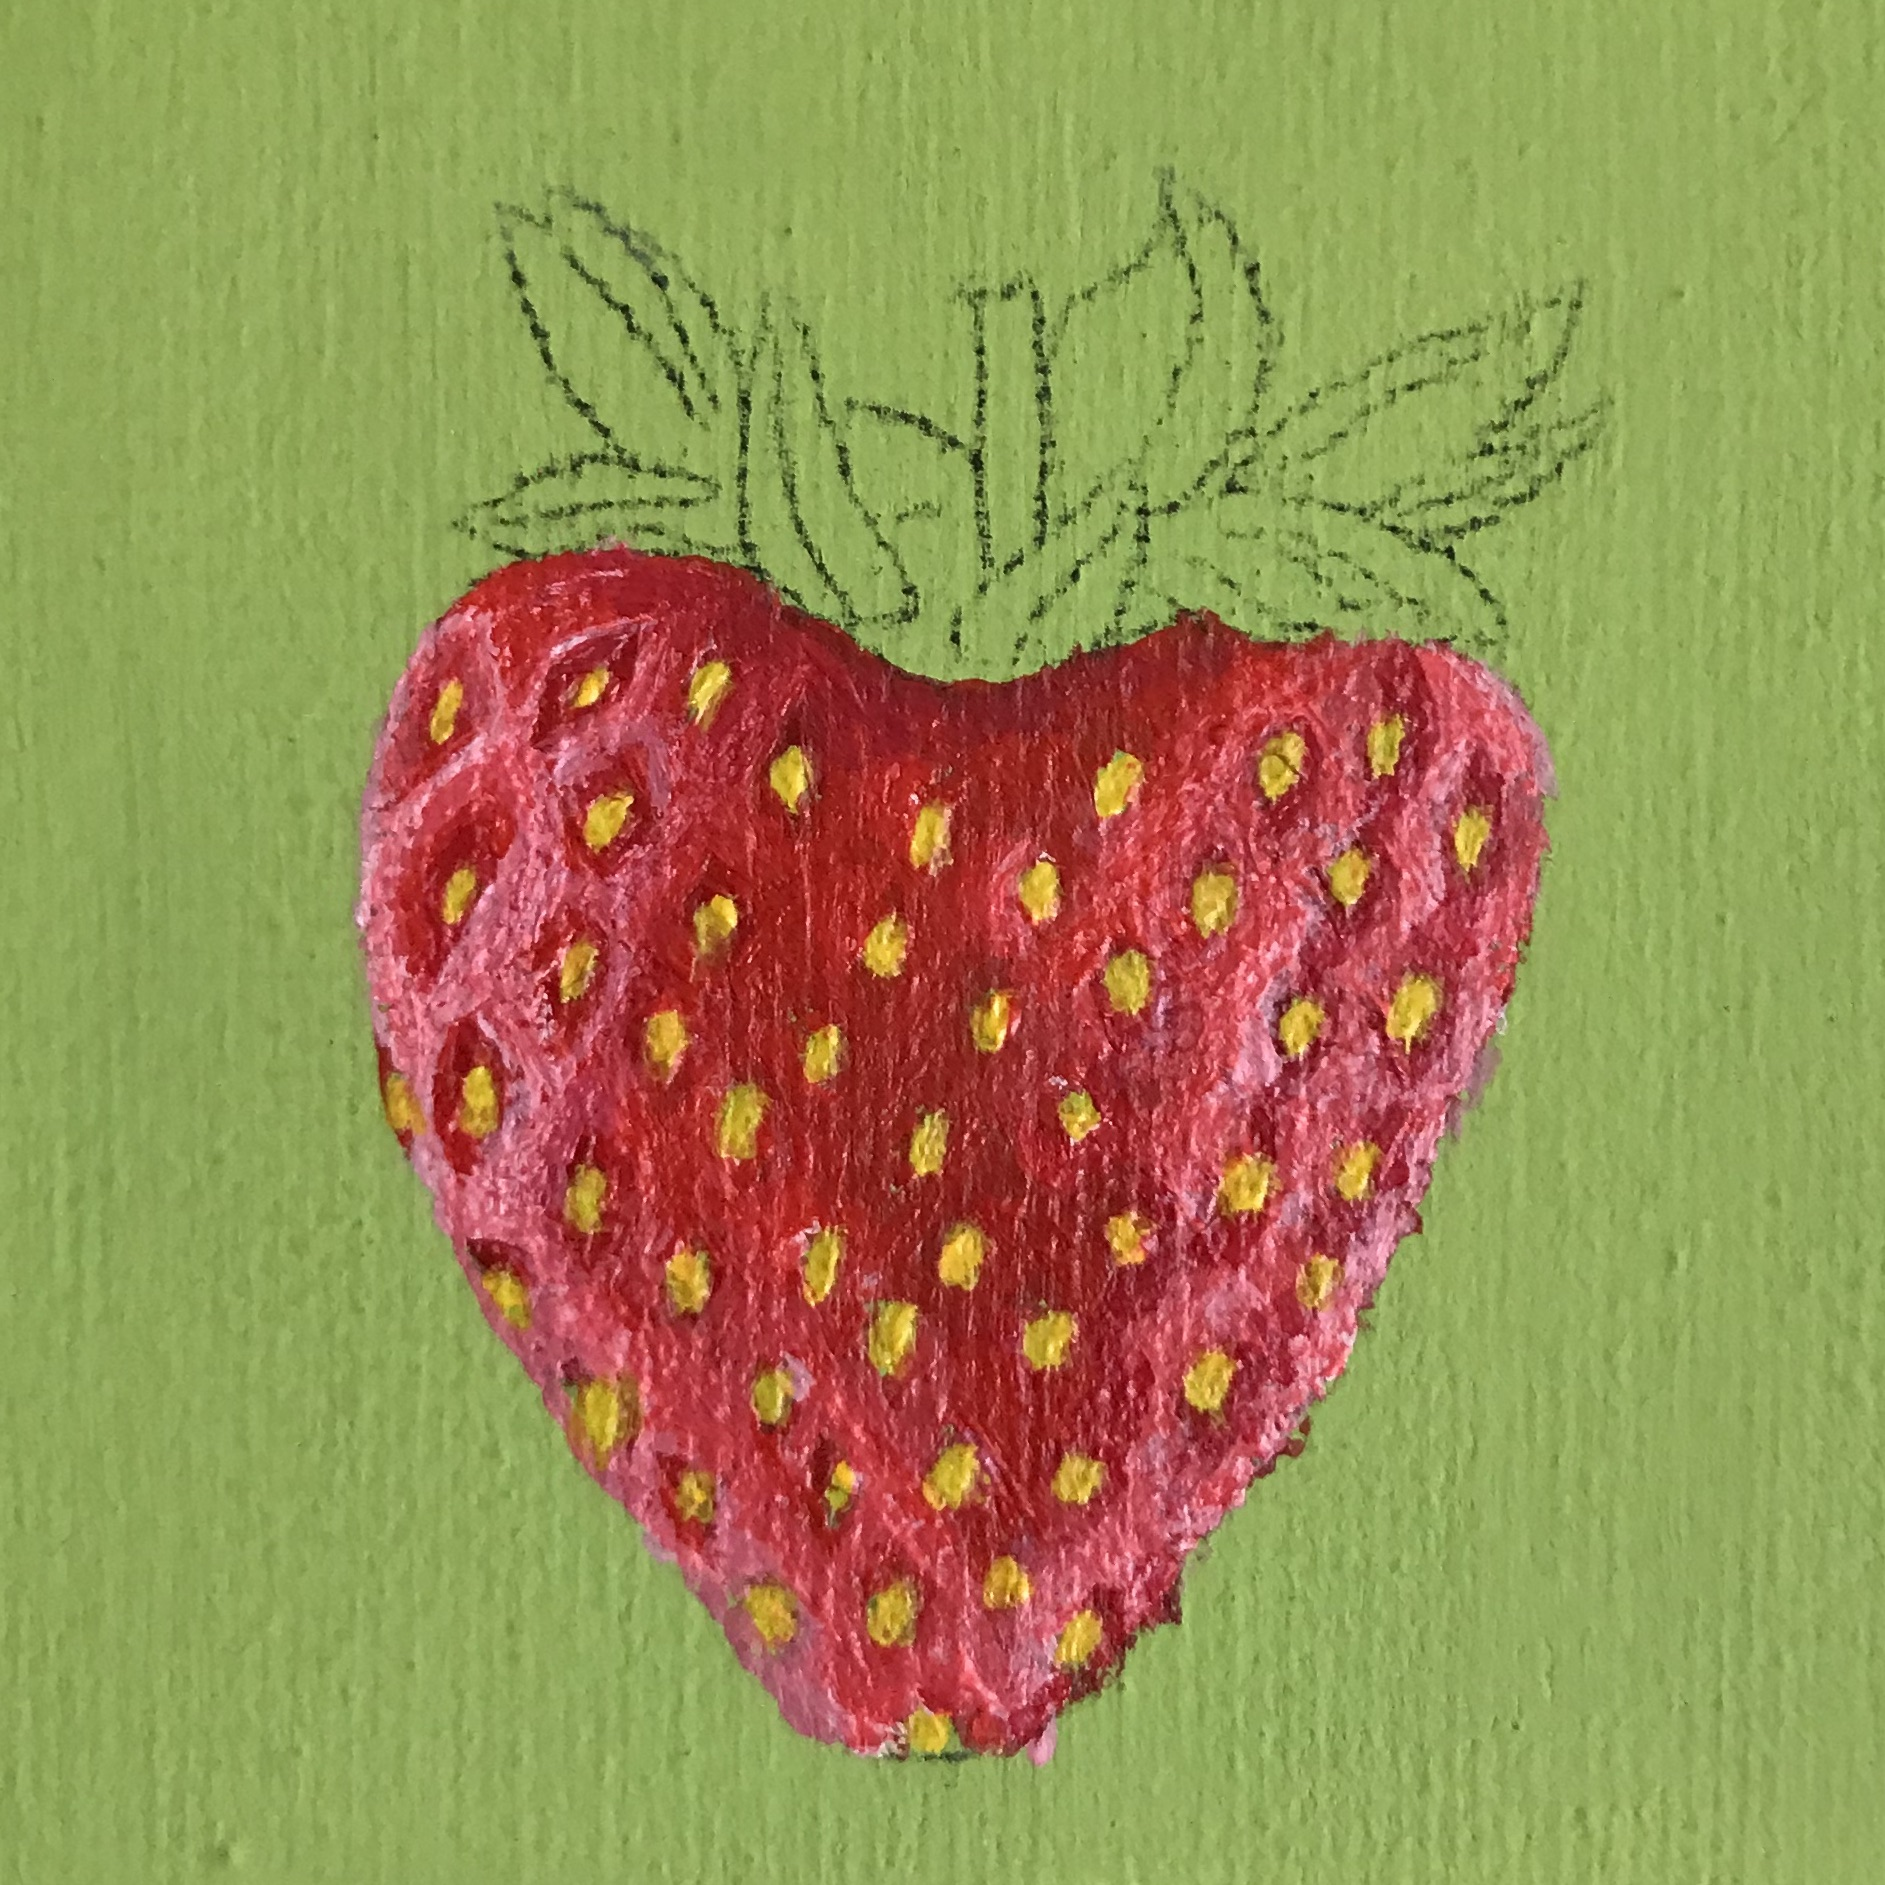
\includegraphics[width=.22\linewidth]{figures/visionscience/fresa_5.jpg}
    6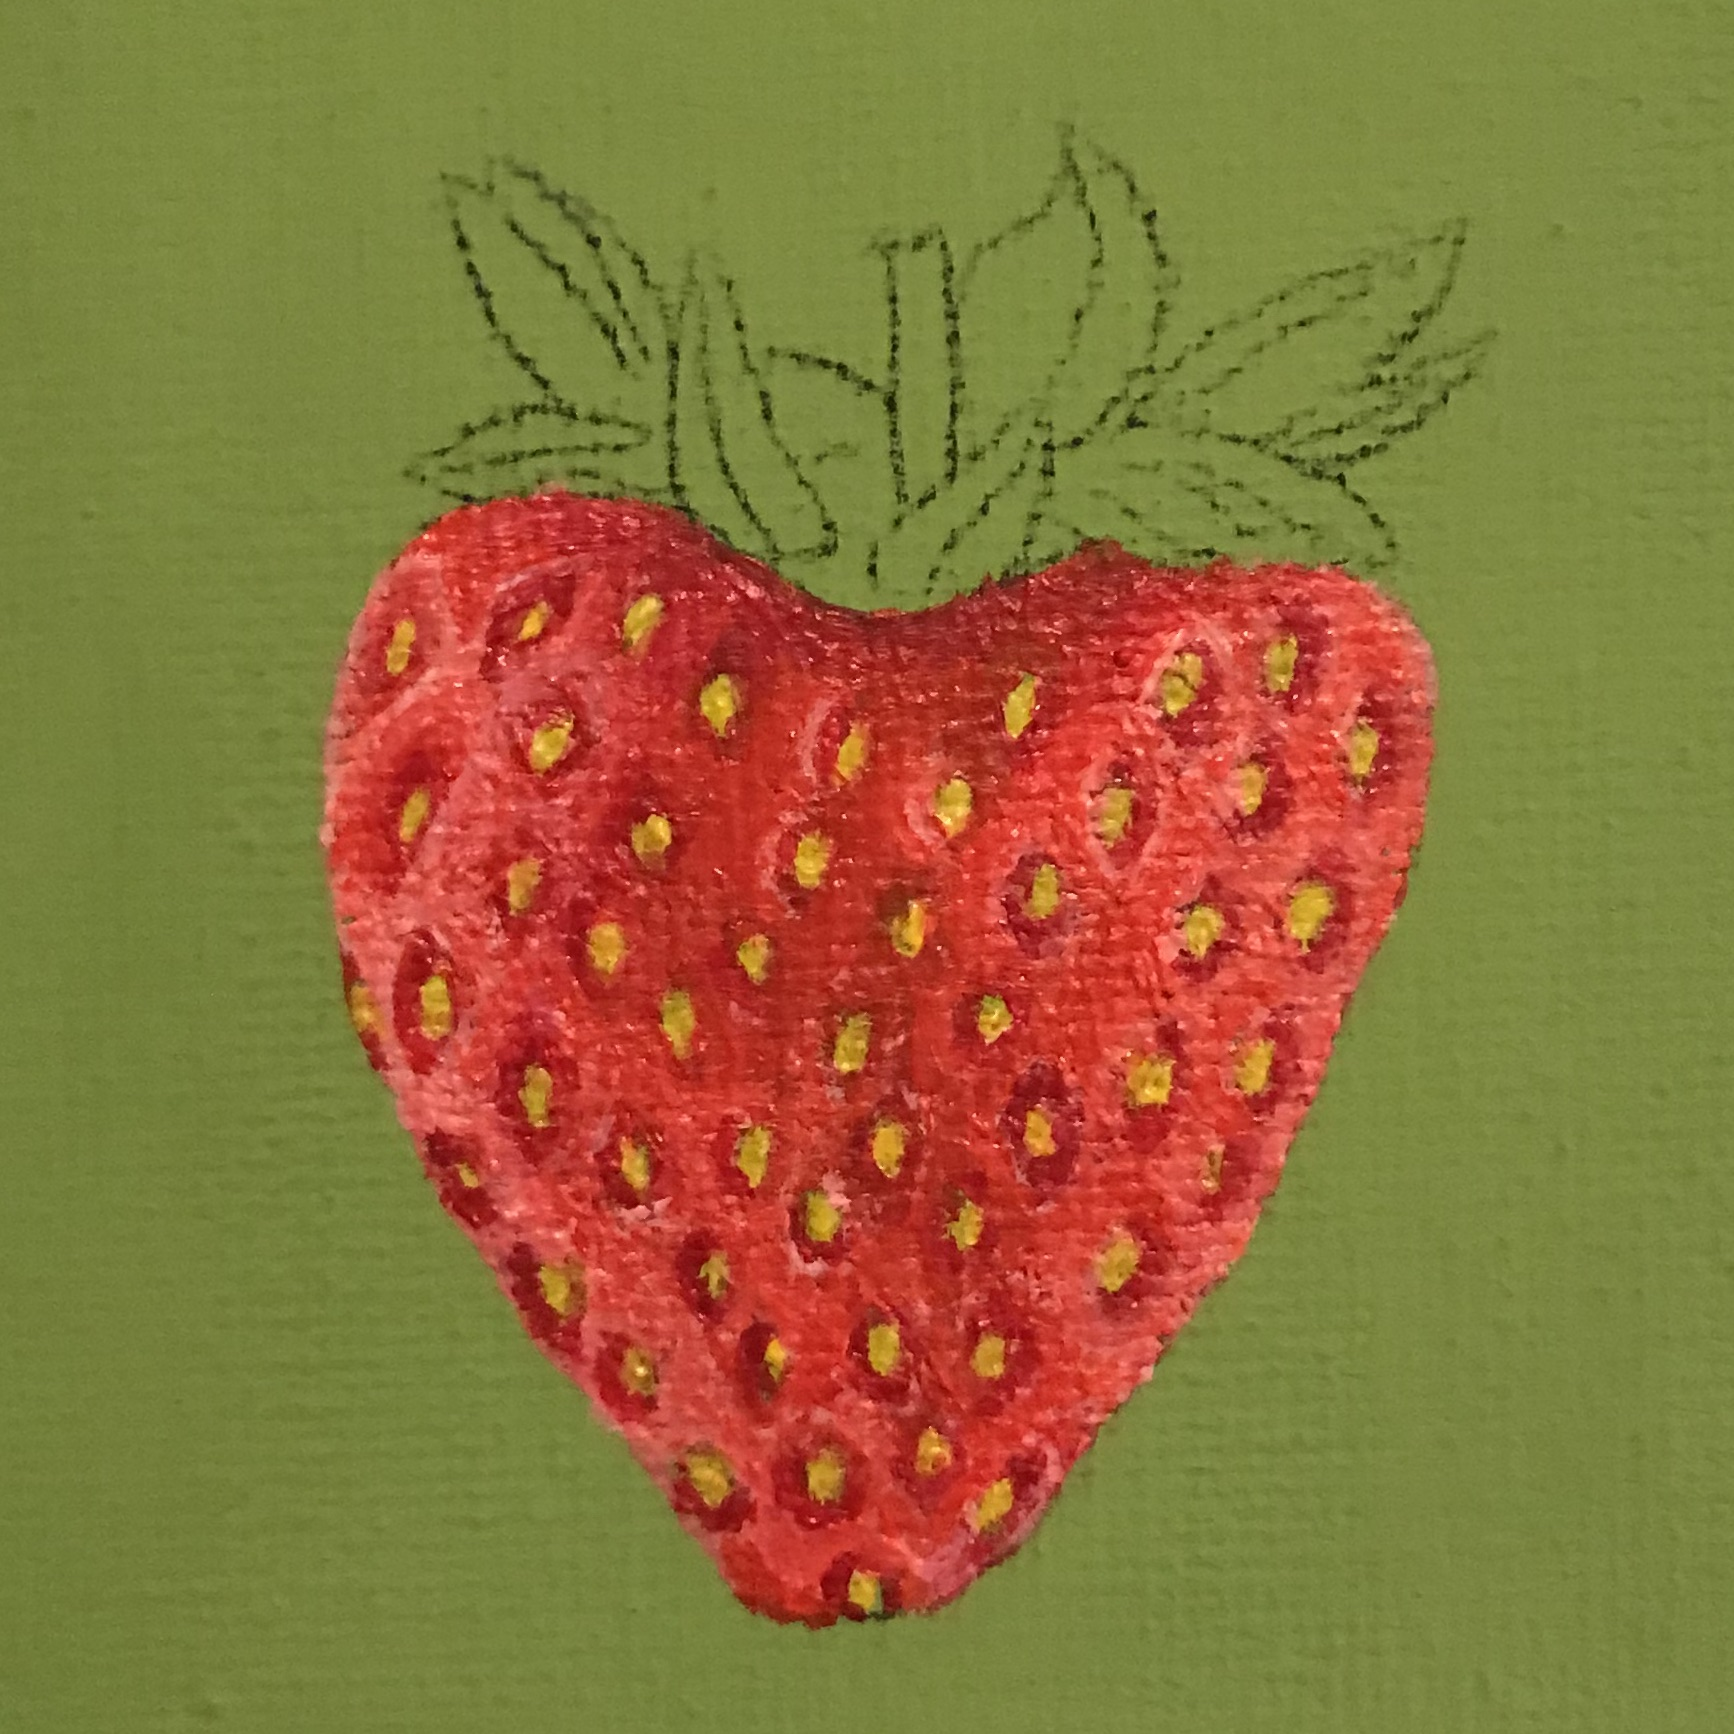
\includegraphics[width=.22\linewidth]{figures/visionscience/fresa_6.jpg}
    7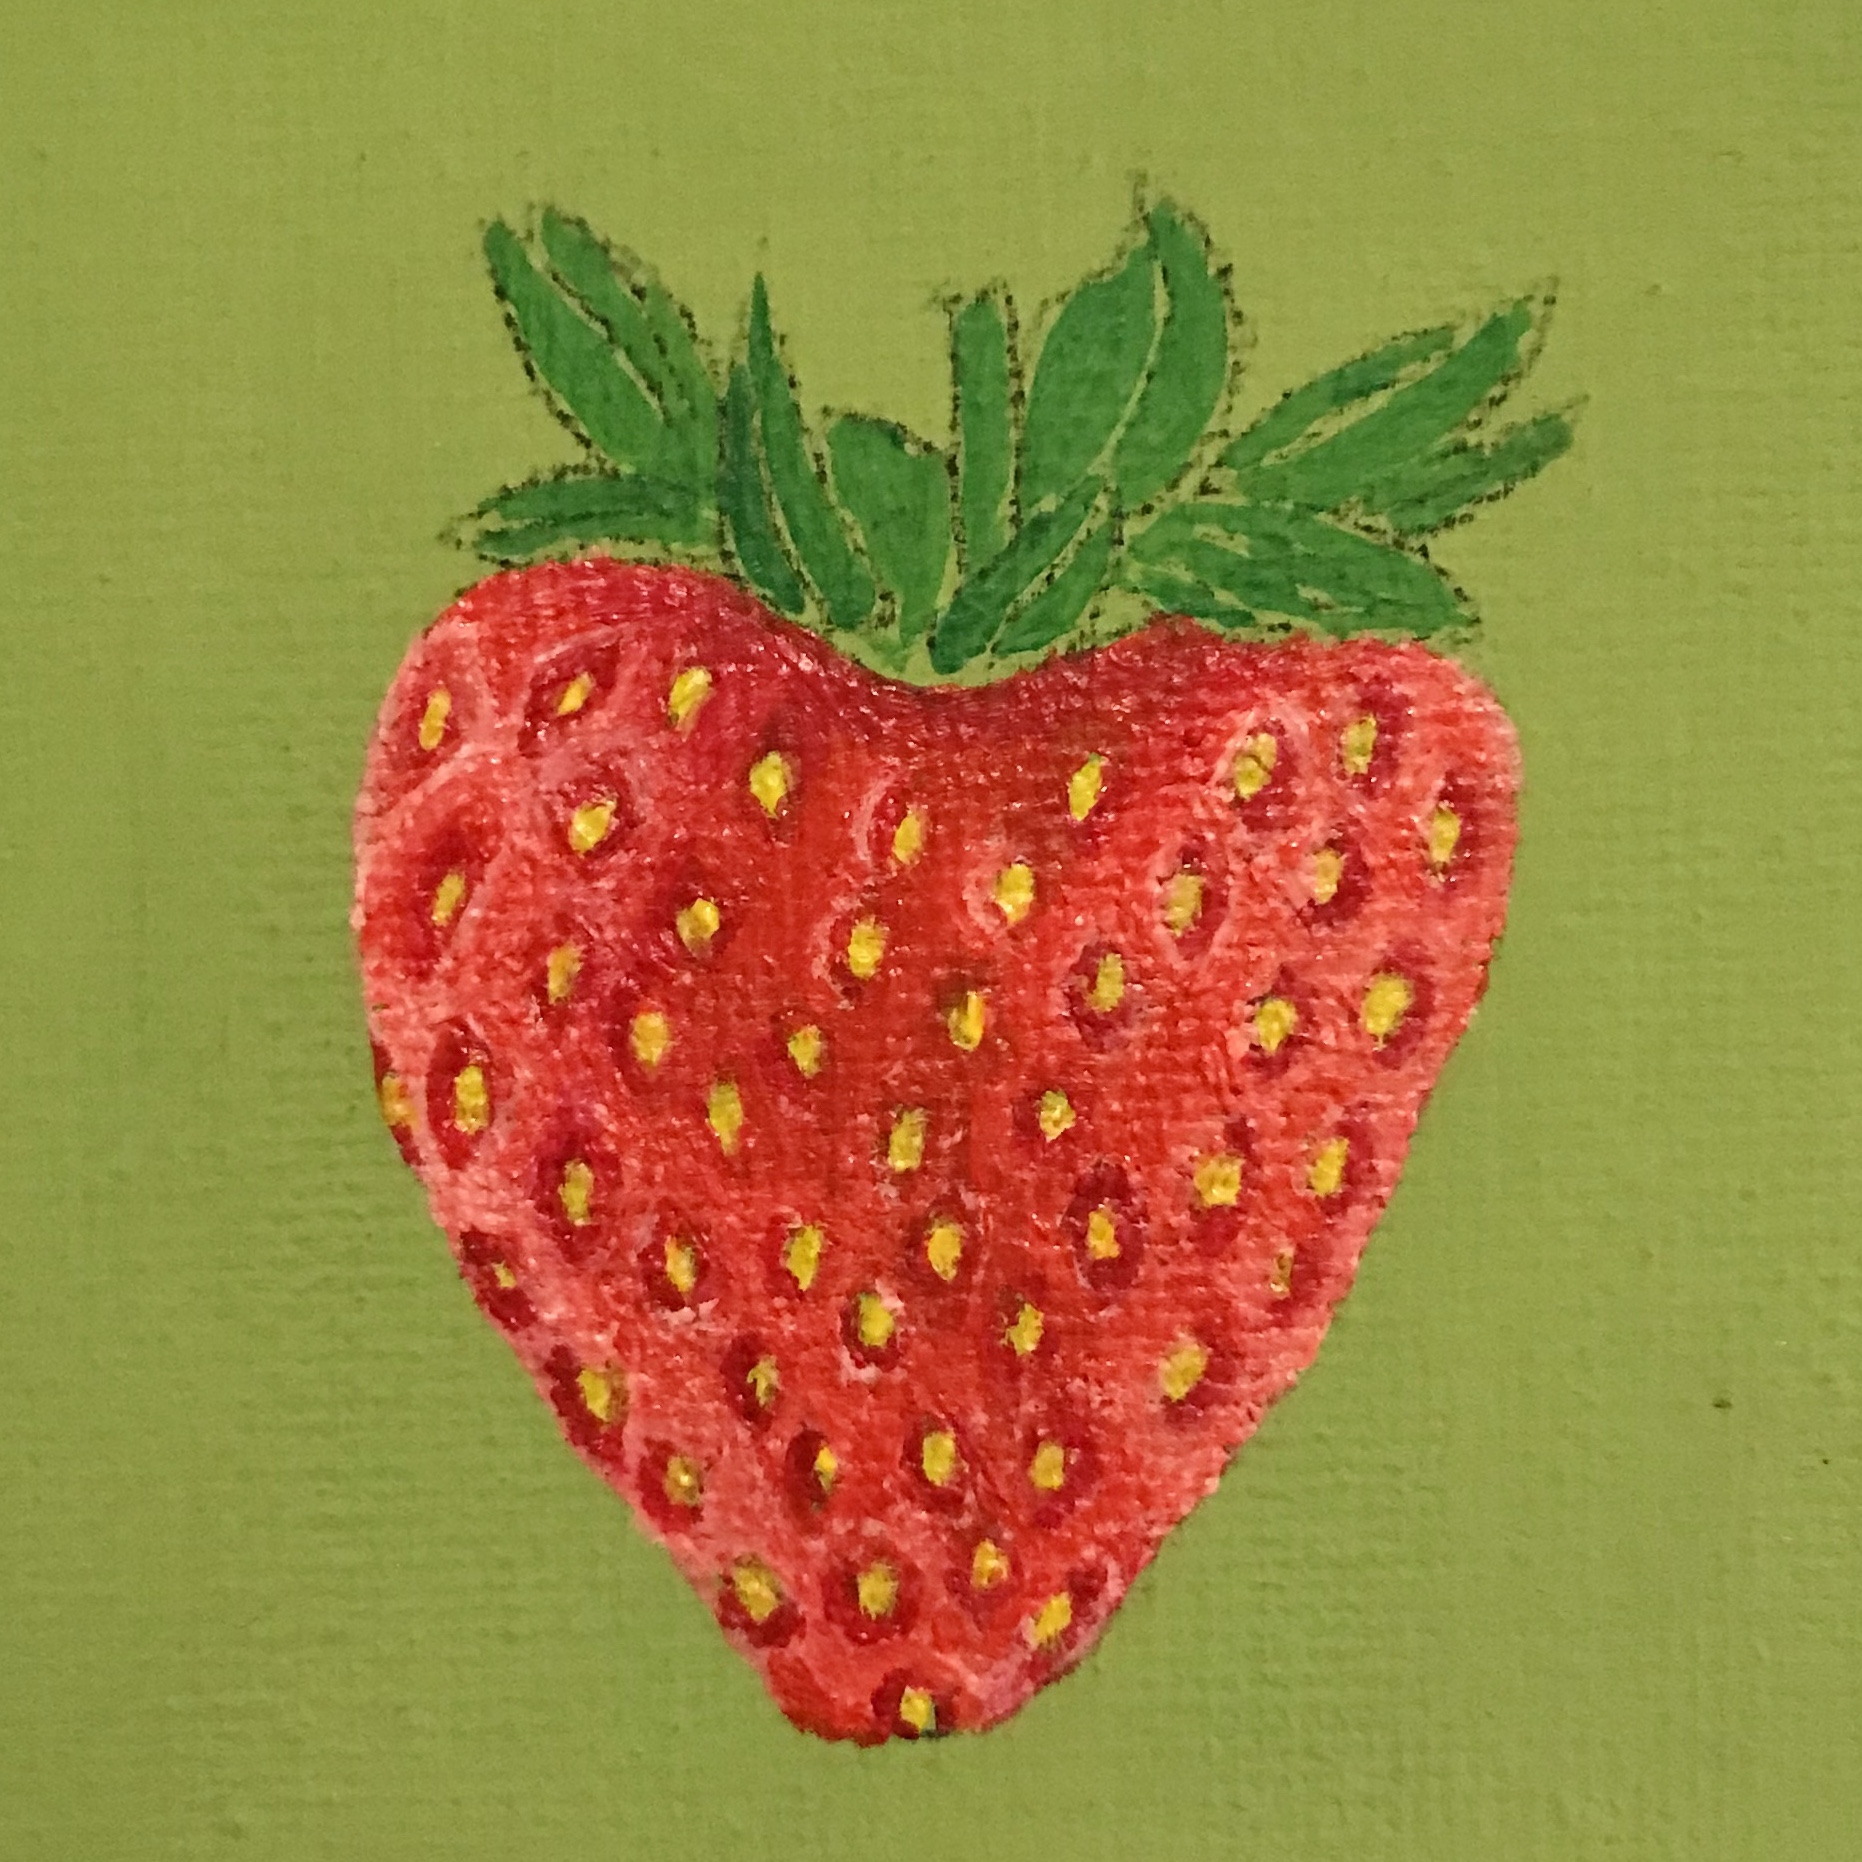
\includegraphics[width=.22\linewidth]{figures/visionscience/fresa_7.jpg}
    8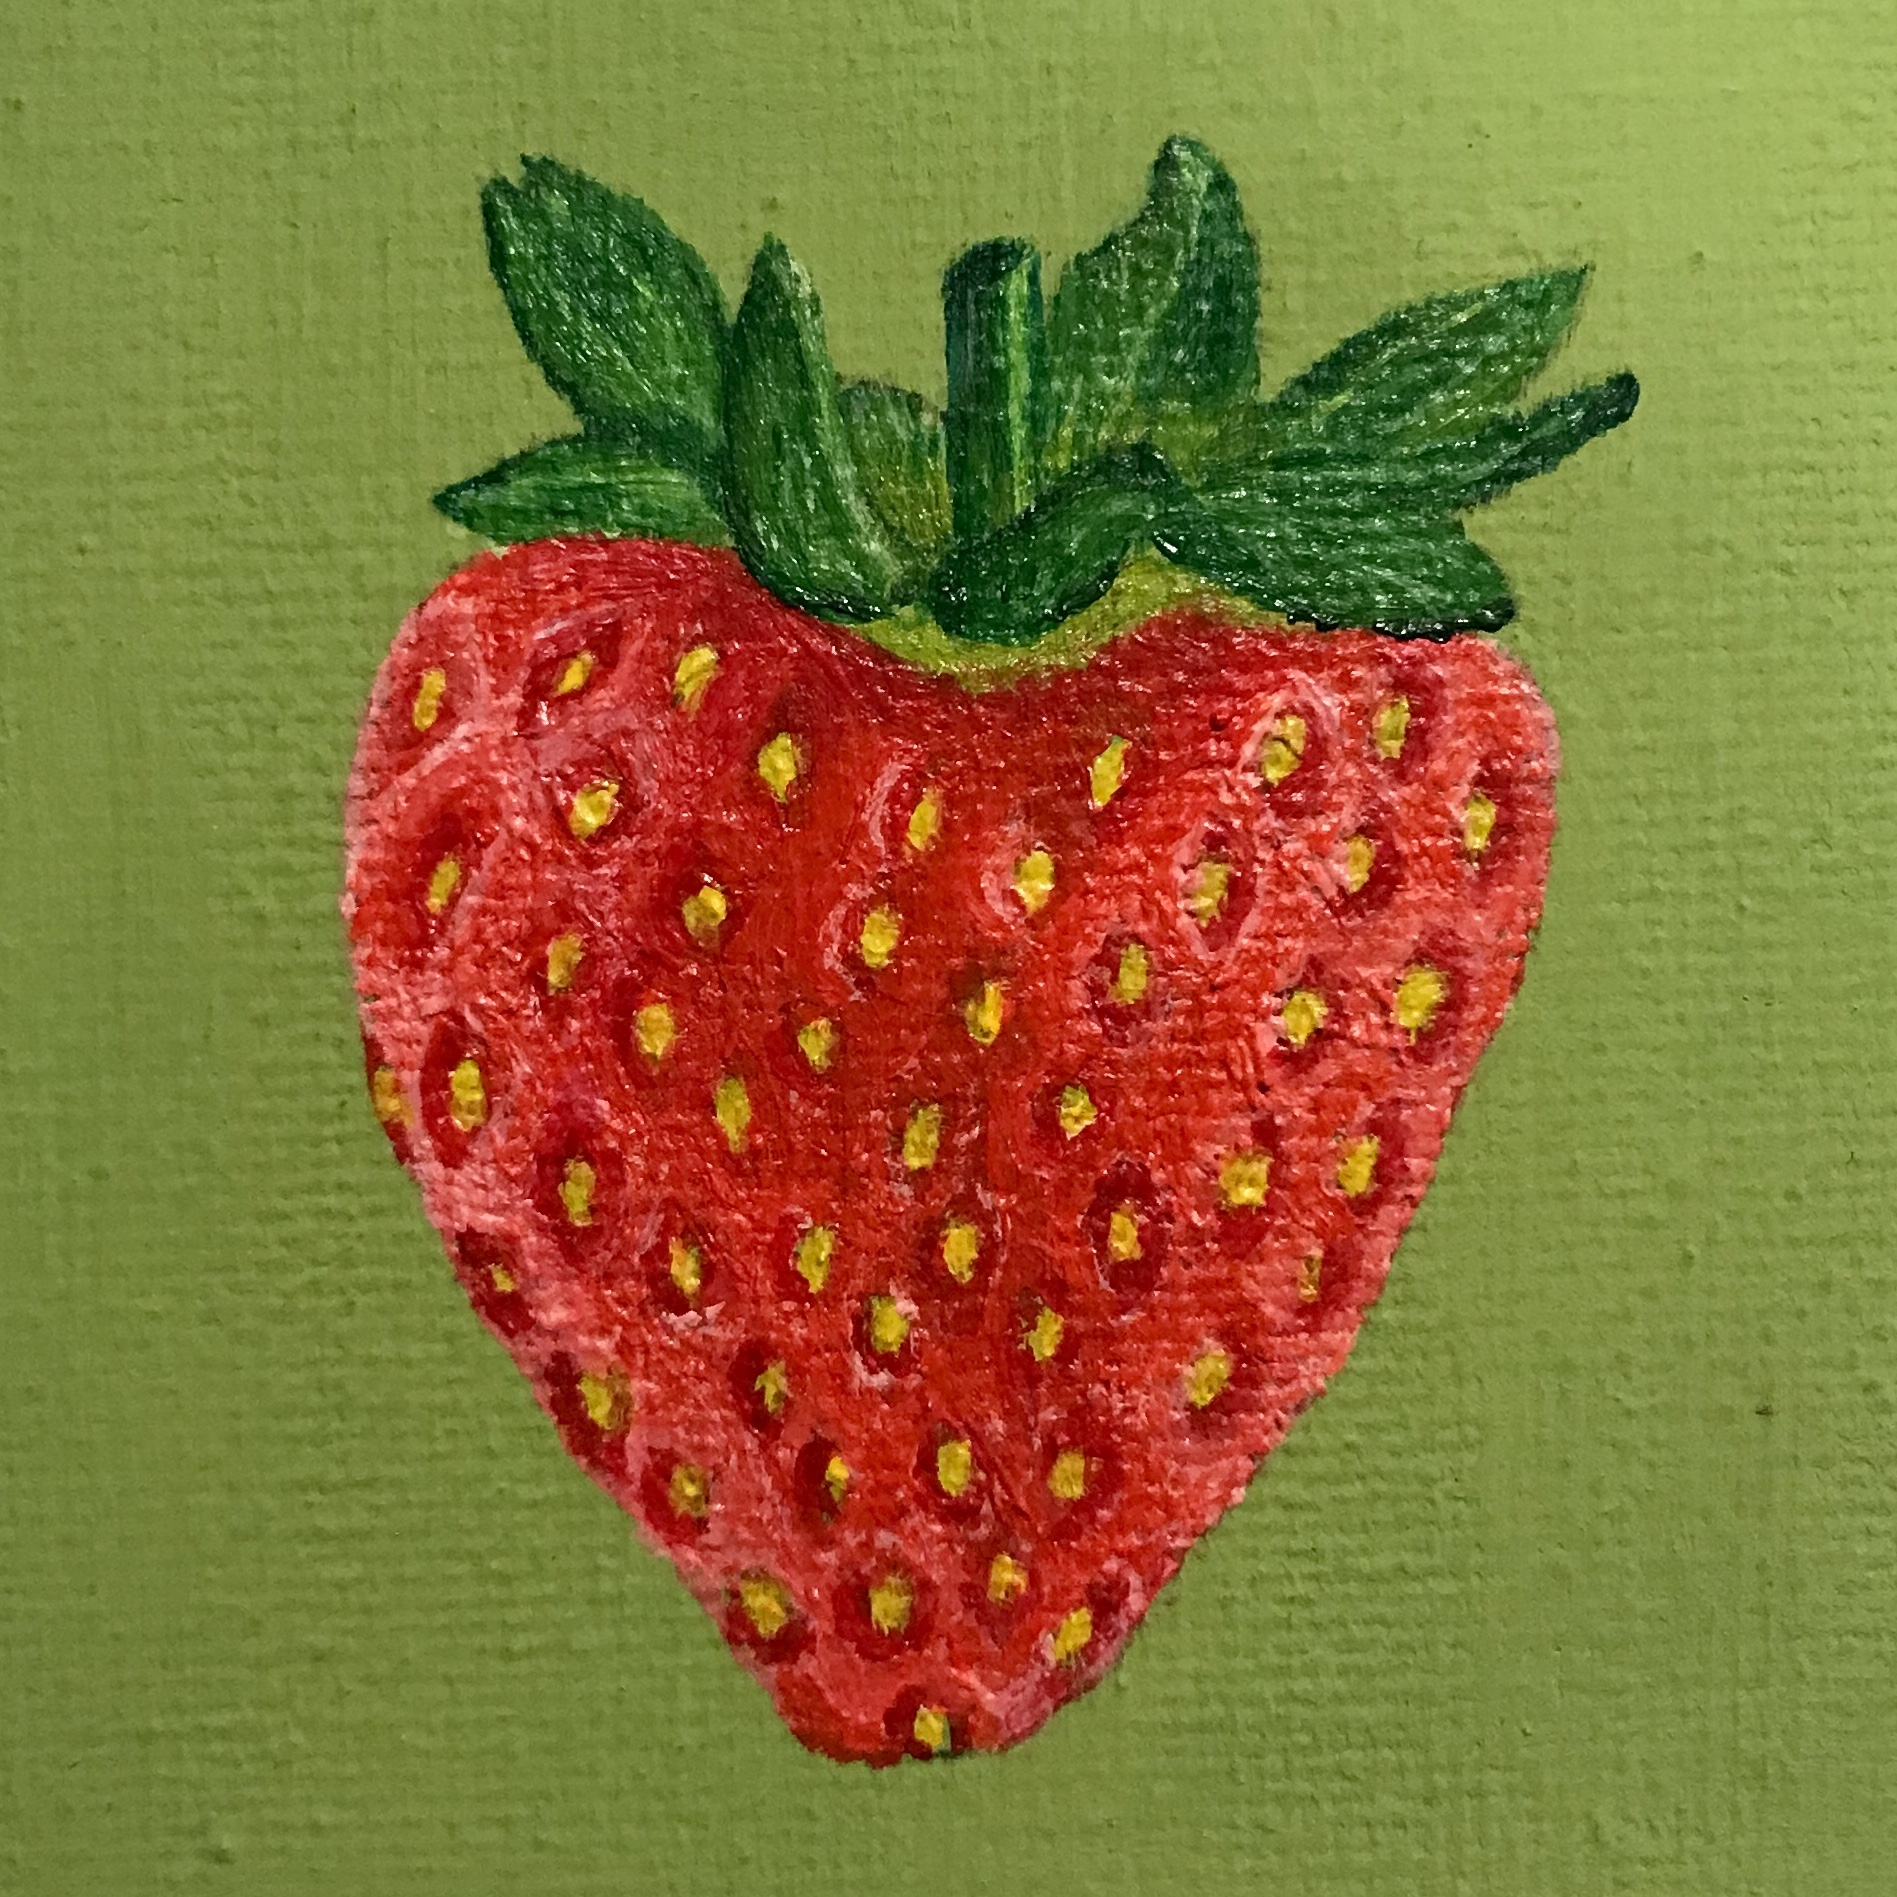
\includegraphics[width=.22\linewidth]{figures/visionscience/fresa_8.jpg} % Photo by Antonio Torralba
    }
    \caption{The following sequence shows different steps in the process of painting a strawberry. {\em Source}: Original images by Agata Lapedriza.}
    \label{fig:agata_painting}
\end{figure}


% \section{Every photo contains thousands of tiny images}
% The image below contains a million pixels, and each is a tiny image.

% \begin{center}
%     patch : image :: image : dataset
% \end{center}

% A common trick in computer vision is to take a method that was developed for processing a \textit{dataset} and instead apply it to the set of patches in an image, or vice versa.


\section{Tree Shadows and Image Formation}

When walking under the shadow of a tree on a bright sunny day when the sun is right above us (\fig{\ref{fig:tree_pinholes}}[left]), we can see how some light rays get through the holes left between leaves, creating spots on the floor (\fig{\ref{fig:tree_pinholes}}[right]). 


\begin{figure}[h!]
\centerline{
    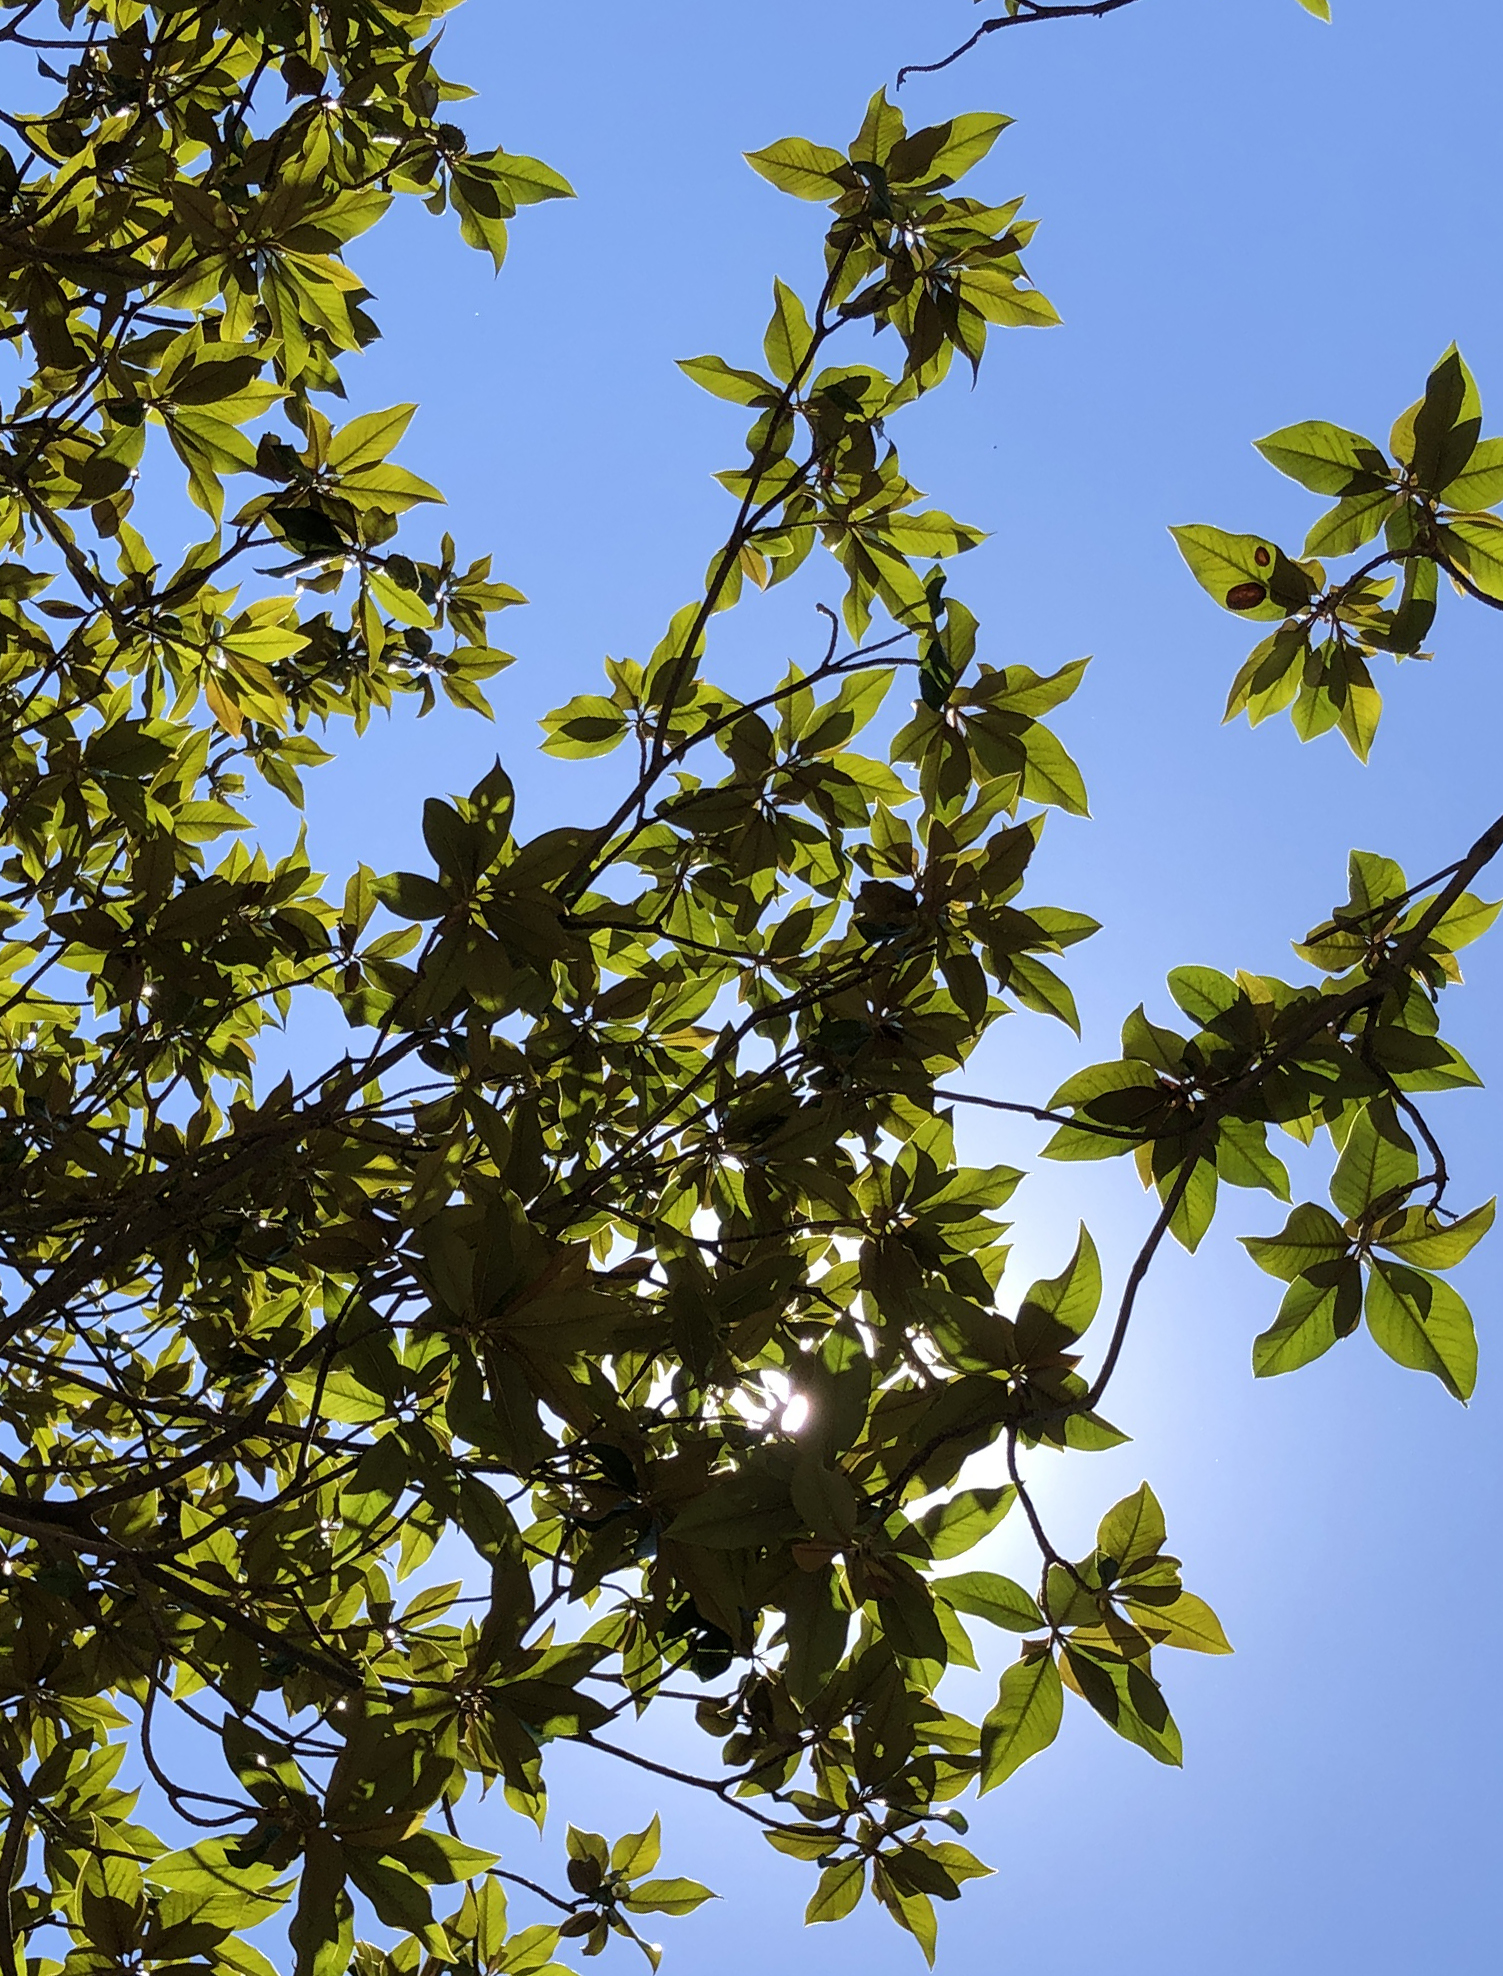
\includegraphics[width=.497\linewidth]{figures/visionscience/IMG_2842_tree_pinholes.jpg} % Photo by Antonio Torralba
    ~~\includegraphics[width=.491\linewidth]{figures/visionscience/IMG_2837_tree_shadow.JPG} % Photo by Antonio Torralba
}
\caption{The shadow of this tree on a normal day projects dozens of pictures of the sun on the ground.}
\label{fig:tree_pinholes}
\end{figure}

But something is a bit odd about the shape of the bright spots projected on the floor. We would expect that the spots of light would have irregular shapes as the openings between leaves will have all kinds of irregular profiles (\fig{\ref{fig:tree_pinholes}}[left]). Instead, as shown in \fig{\ref{fig:tree_pinholes}}(right), the spots appear to be circular and of similar size. This observation already puzzled Aristotle. What could be happening?  As a hint, \fig{\ref{fig:tree_shadow_eclipse}} shows the shadow of leaves during a solar eclipse.


\begin{figure}[h!]
\centerline{
    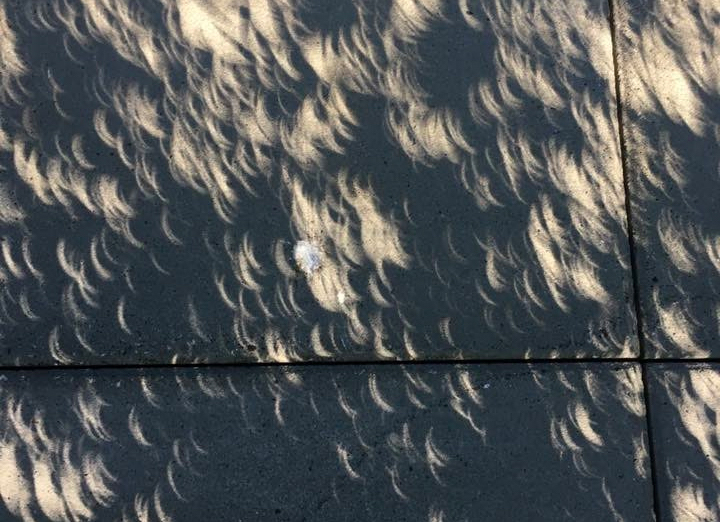
\includegraphics[width=.9\linewidth]{figures/visionscience/tree_shadow_eclipse2.jpg} % Photo by Bill Freeman
}
\caption{During an eclipse, the shadow of the tree contains many copies of the crescent sun.}
\label{fig:tree_shadow_eclipse}
\end{figure}


One of the most common situations that we often encounter is the {\bf pinhole cameras} formed by the spacing between the leaves of a tree. 
\index{Camera!Pinhole camera}
The tiny
holes between the leaves of a tree create a multitude of pinholes. The pinholes created by the leaves project different
copies of the sun on the floor. When the openings between leaves are small enough, the shape of the projected spot light is dominated by the shape of the sun.
This is something we see often but rarely think about the origin of the spotlights that we
see on the floor. 


%\centerline{
%    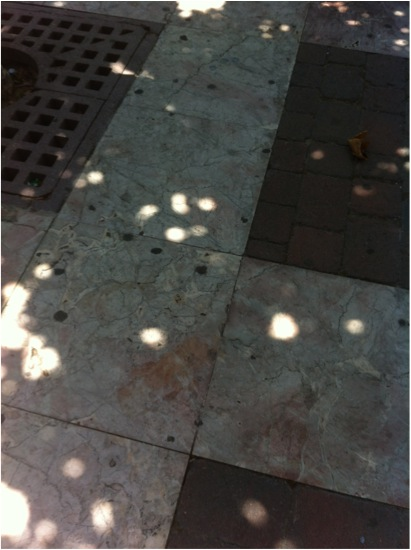
\includegraphics[width=.6\linewidth]{figures/visionscience/trees.jpg}}
    
    
In fact, the leaves of a tree create pinholes that produce images in many other situations. We will talk about pinhole cameras in \chap{\ref{chapter:imaging}}.

\section{Horizontal or Vertical}

Looking at the previous picture of the shadow of the tree, another interesting question comes to mind: How do you know you are looking at a picture of the ground? How do you know the orientation of the camera?

Look at the two drawings in \fig{\ref{fig:vertical_or_horizontal}}. The lines in the drawing on the left correspond to tiles in a floor, the line drawing on the right is the same drawing rotated 90 degrees. Which one seems to be an horizontal surface and which one seems vertical? Why? The differences in the line orientations are subtle and yet it produces a very different perception.

\begin{figure}[t]
\centerline{
    \includegraphics[width=1\linewidth]{figures/visionscience/vertical_or_horizontal.eps}}
    \caption{Line drawings. The one on the left seems to correspond to an horizontal surface while the one on the right looks like a vertical surface.}
    \label{fig:vertical_or_horizontal}
\end{figure}

In the arrangement in the left, there are two {\bf vanishing points} (the points in which parallel lines intersect) and both are above the drawing, compatible with the horizon line. However, on the drawing on the right, one of the vanishing points is below the figure and gives the impression that the camera is looking at a vertical wall (the camera seems to be higher than the visible part of the wall). The horizon line of the plane (the line that connects both vanishing points) is horizontal in the left drawing and vertical on the right one.

%\section{The geometry of vision}




\section{Motion Blur}

When we are in a moving car and we take a picture from the passenger window, often images will appear blurring, specially when taken at night (\fig{\ref{fig:Paris_from_moving_car}}). Blur is due to the fact that the camera sensor is collecting light during a period of time while the car is moving and the picture that results is the average of several translated copies of the same image. However, note that not all of the objects are equally blurry. Things that are far away might still look sharp while things nearby appear very blurry.  

\begin{figure}[h!]
\centerline{
    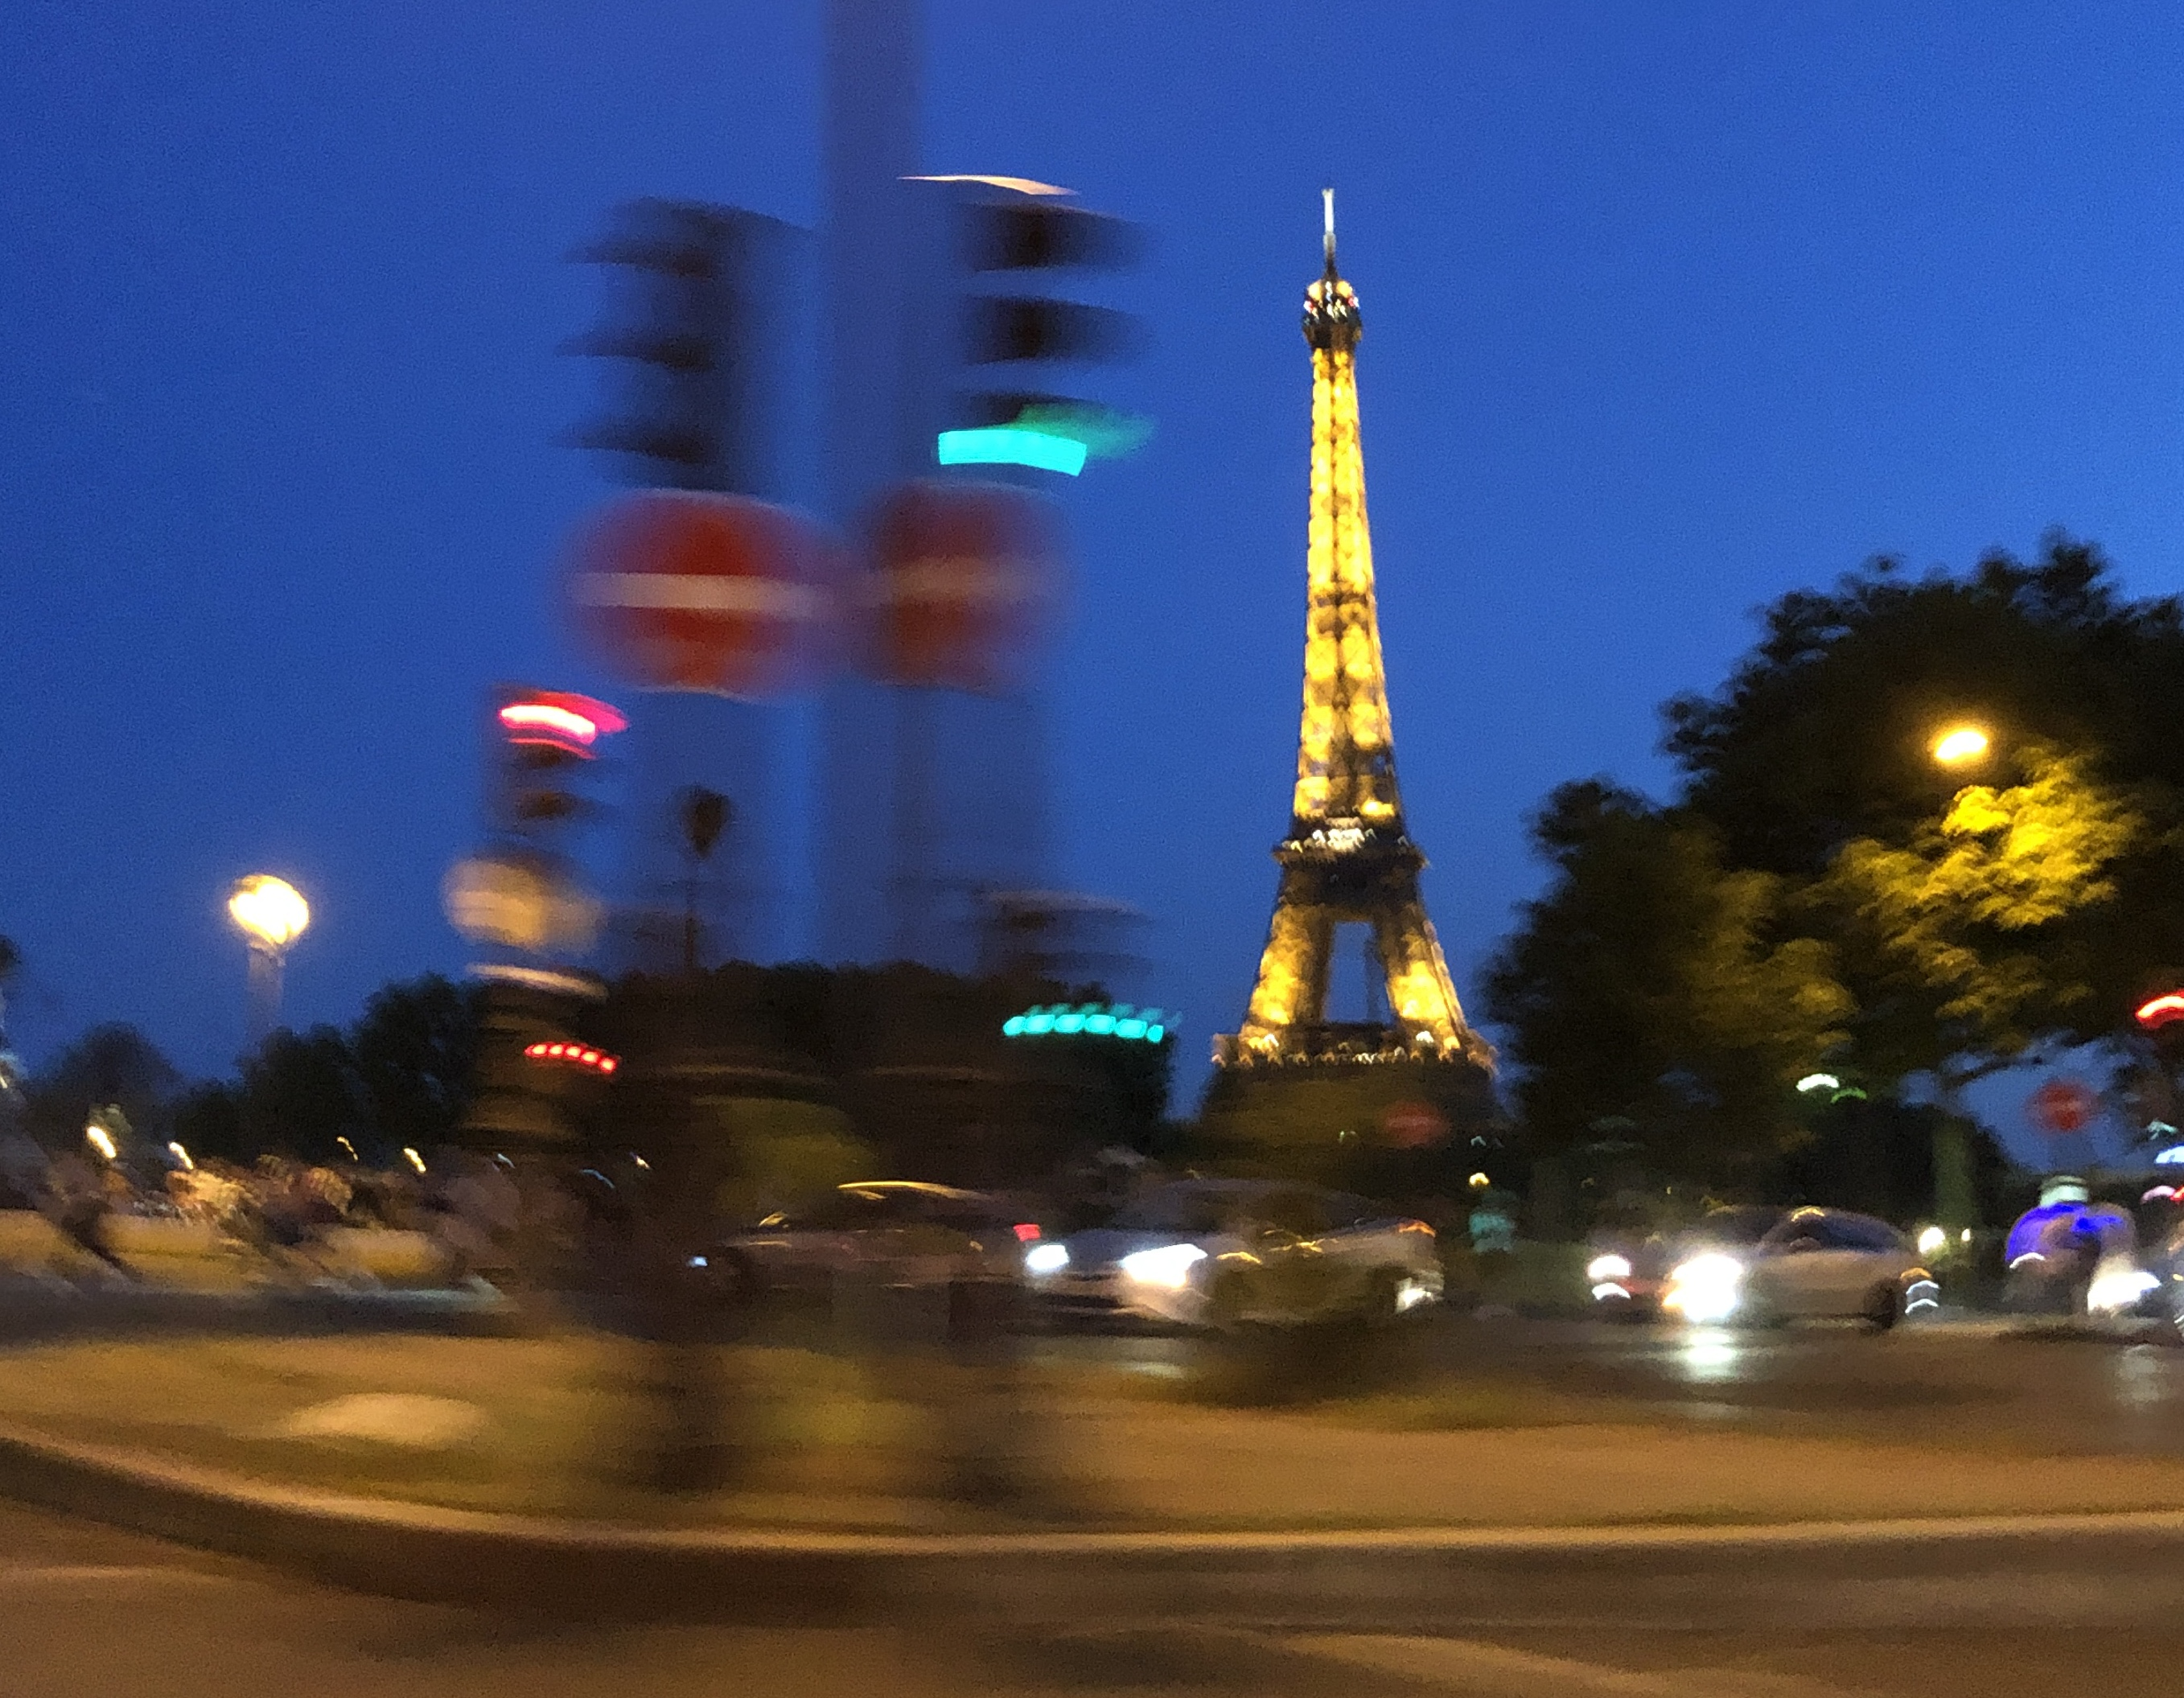
\includegraphics[width=1\linewidth]{figures/visionscience/motion_blur.jpg}} % Photo by Antonio Torralba
    \caption{Picture of Paris taken from a moving car.}
    \label{fig:Paris_from_moving_car}
\end{figure}

The amount of blur is related to the car speed, the exposure time, and the distance between the camera and each object in the scene. We will talk more about how camera motion relates to distance in \chap{\ref{chapter:3D_motion_and_its_2D_projection}}.

\section{Accidents Happen}

\marginnote{Principle of continuity.
In the following drawing, we see one wave and one line:
\\[6pt]
\centerline{
\includegraphics[width=.6\linewidth]{figures/visionscience/principle_continuity_1.eps}}
\\[6pt]
Despite this, other 
groupings are also 
possible.
\\[6pt]
\centerline{
\includegraphics[width=.6\linewidth]{figures/visionscience/principle_continuity_2.eps}}
}
We learned about the generic view principle in \chap{\ref{chapter:simplesystem}}, and this idea comes up a lot in computer vision. But it turns out that in most photographs it's easy to find accidents. This is because photos contain so many things, thousands of tiny images, and there are so many coincidences that could occur. \Fig{\ref{fig:visionscience:migrant_mother}} shows a famous photo and we will look for some coincidences in it. The coincidences are of a specific variety: generically, if you see smooth, continuous line segments you assume that they lie on a single object because it's quite a coincidence for two objects to line up just so their contours perfectly align. The gestalt psychologists called this the {\bf principle of continuity}. The insets  for \fig{\ref{fig:visionscience:migrant_mother}} show several locations in the photo ``Migrant Mother'' by Dorothea Lange where exactly this happens. Can you find more?

\begin{figure}[h!]
\centerline{
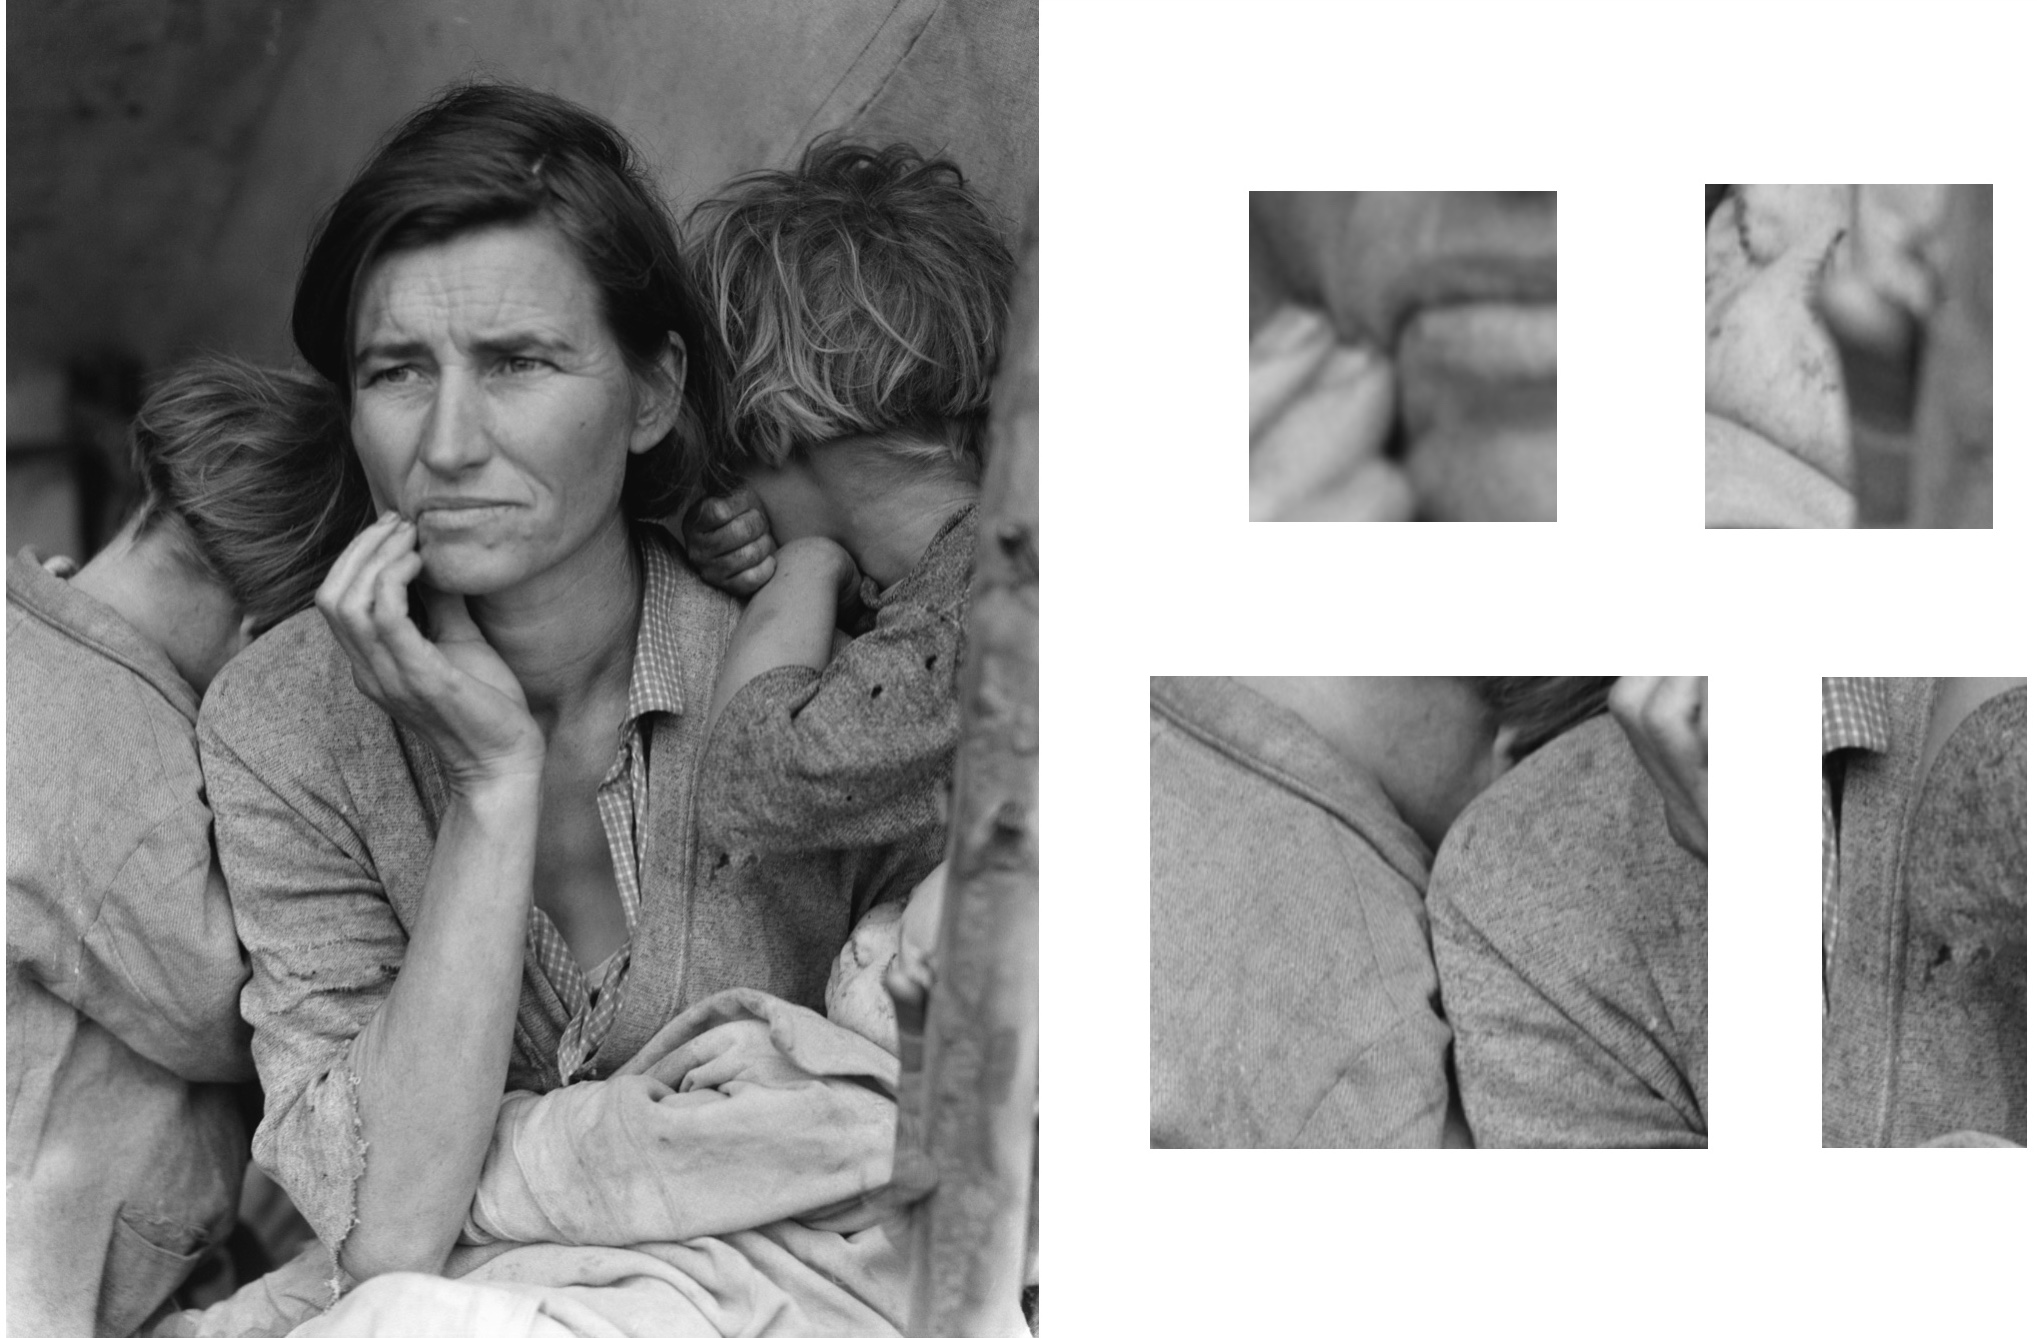
\includegraphics[width=1\linewidth]{figures/visionscience/accidents_migrant_mother.jpg}}
\caption{Source: Migrant Mother (1936), by Dorothea Lange. On the right are four examples of coincidences that violate the Gestalt principle of continuity. From top-left clockwise: finger boundary aligns with lip contour, cloth aligns with eye, creases align on two different shirts, sleeve boundary is tangent to line on a different shirt.}
\label{fig:visionscience:migrant_mother}
\end{figure}
% image source: https://en.wikipedia.org/wiki/File:Lange-MigrantMother02.jpg
% license: public domain

You have to be careful about this when developing vision algorithms. If you assume \textit{no} accidents will happen, then you will be in for some trouble. This is one reason why older, rule-based methods failed, because they did not handle exceptions to the rules.




\section{Cues for Support}

When can we tell by looking that one object supports another?  Consider the ball over a surface depicted in \fig{\ref{fig:cues_for_suppport}}.  The drop shadow provides a strong cue that the ball is above the surface in figures \ref{fig:cues_for_suppport}(a) and \ref{fig:cues_for_suppport}(c), while the slack string provides evidence for the ball being on the surface in figures \ref{fig:cues_for_suppport}(b) and \ref{fig:cues_for_suppport}(c).  
Only \fig{\ref{fig:cues_for_suppport}}{c} is a doctored photograph.

In which of these figures does the ball appear to be in contact with the ground plane?

\begin{figure}[h!]
\centerline{
\sublabel{a}{ \includegraphics[width=0.47\linewidth]{figures/visionscience/ballUp.jpg}}
    \sublabel{b}{\includegraphics[width=0.47\linewidth]{figures/visionscience/ballDown.jpg} }
    }
  \centerline{
    \sublabel{c}{\includegraphics[width=0.47\linewidth]{figures/visionscience/ballPuzzle.jpg}}
    }
    \caption{Cues for support. The relative location between an object, and its shadow on the ground is a powerful cue for contact.}
    \label{fig:cues_for_suppport}
\end{figure}
% image source: photos by Bill


\section{Looking at Raindrops}

When it rains you get to see a rare sight. Every raindrop refracts a panorama of the scene around it (\fig{\ref{fig:droplets}}). What you are seeing is not just one photo but hundreds of images of the scene, one in each raindrop, all from slightly different angles. It turns out specially designed cameras have been made that do the same thing, and they are called {\bf light field cameras}.
\index{Camera!Light field cameras}
These cameras use an array of tiny lenses rather than raindrops, but the result is similar: they capture what the scene looks like from hundreds of different viewing angles, and from that density of information they can achieve many interesting tricks, such as triangulating the depth of objects in the scene and synthetically refocusing the image after it has been taken.

\begin{figure}[t]
\centerline{
    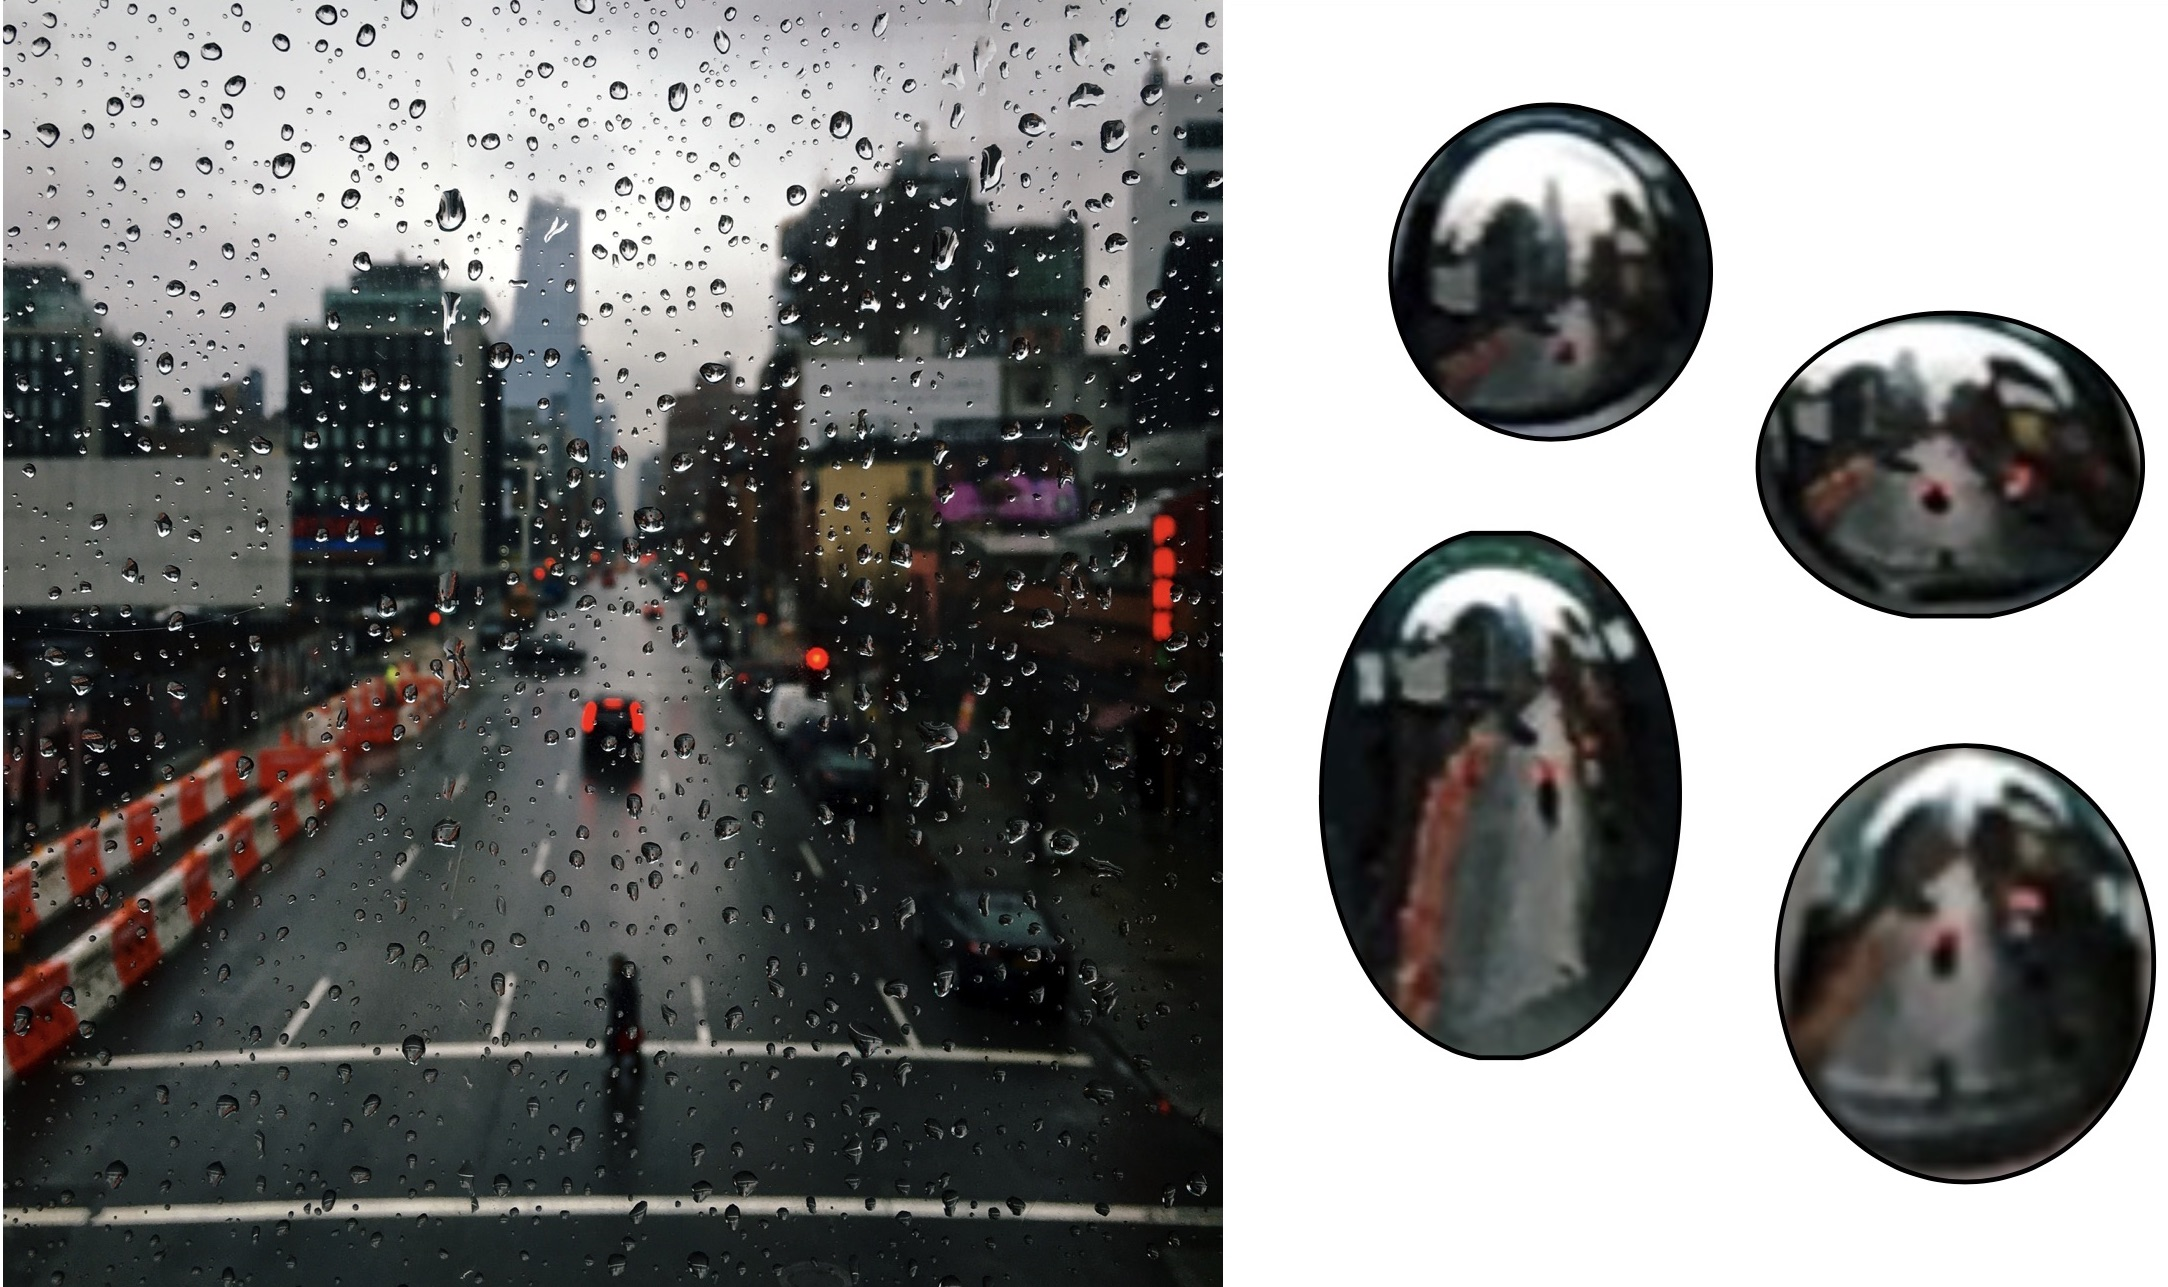
\includegraphics[width=1.0\linewidth]{figures/visionscience/droplets.jpg}}
    \caption{A naturally occurring light field camera. This picture of raindrops on a window contains hundreds of tiny images of the scene, one in each raindrop. The images to the right are individual zoomed in raindrops from the photo on the left.}
    \label{fig:droplets}
\end{figure}
% Photo by Phillip Isola


\section{Plato's Cave}

% \begin{figure}[h]
% \centerline{
%      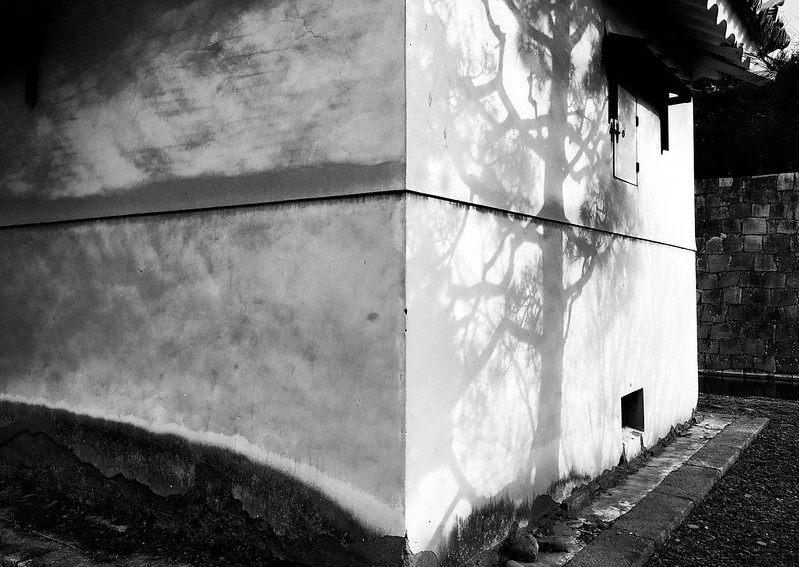
\includegraphics[width=0.8\linewidth]{figures/visionscience/fading_shadows.jpg}}
%      \caption{Vision is analogous to Plato's Allegory of the Cave.  An image is a crude projection of the underlying physical state.}
%  \end{figure}
% % Photo by Phillip Isola

In the \textit{Allegory of the Cave}, Plato imagined a group of prisoners 
chained up in a cave whose only experience of the outside world is through shadows cast on the cave's wall.
When we look at images, we think we are directly seeing reality, but actually the situation is much more like Plato's cave. An image is a crude projection of the underlying physical state. It collapses all the 3D geometry into a flat 2D grid of pixels. From any given viewing angle, most of the scene is occluded. Materials are only depicted in terms of how photons bounce off their surfaces; what's below the surface may be completely omitted. When you look at a picture, think about all the things you cannot see. There's more you don't see than you do. One job of a vision system is to infer everything you can't see given everything you can.

\marginnote{The allegory of the cave has several layers of indirection: the shadows are cast by puppets that are controlled by puppeteers who act out interpretations of the broader reality outside.}

\section{How Do You Know Something Is Wet?}

Our visual system allows us to recognize not just objects, but also material. We can tell if something will feel hot or cold, soft or hard, smooth or rugged. We can also recognize if something is wet or not without touching it, as shown in \fig{\ref{fig:wet_sand}}. 



\begin{figure}[t]
\centerline{
    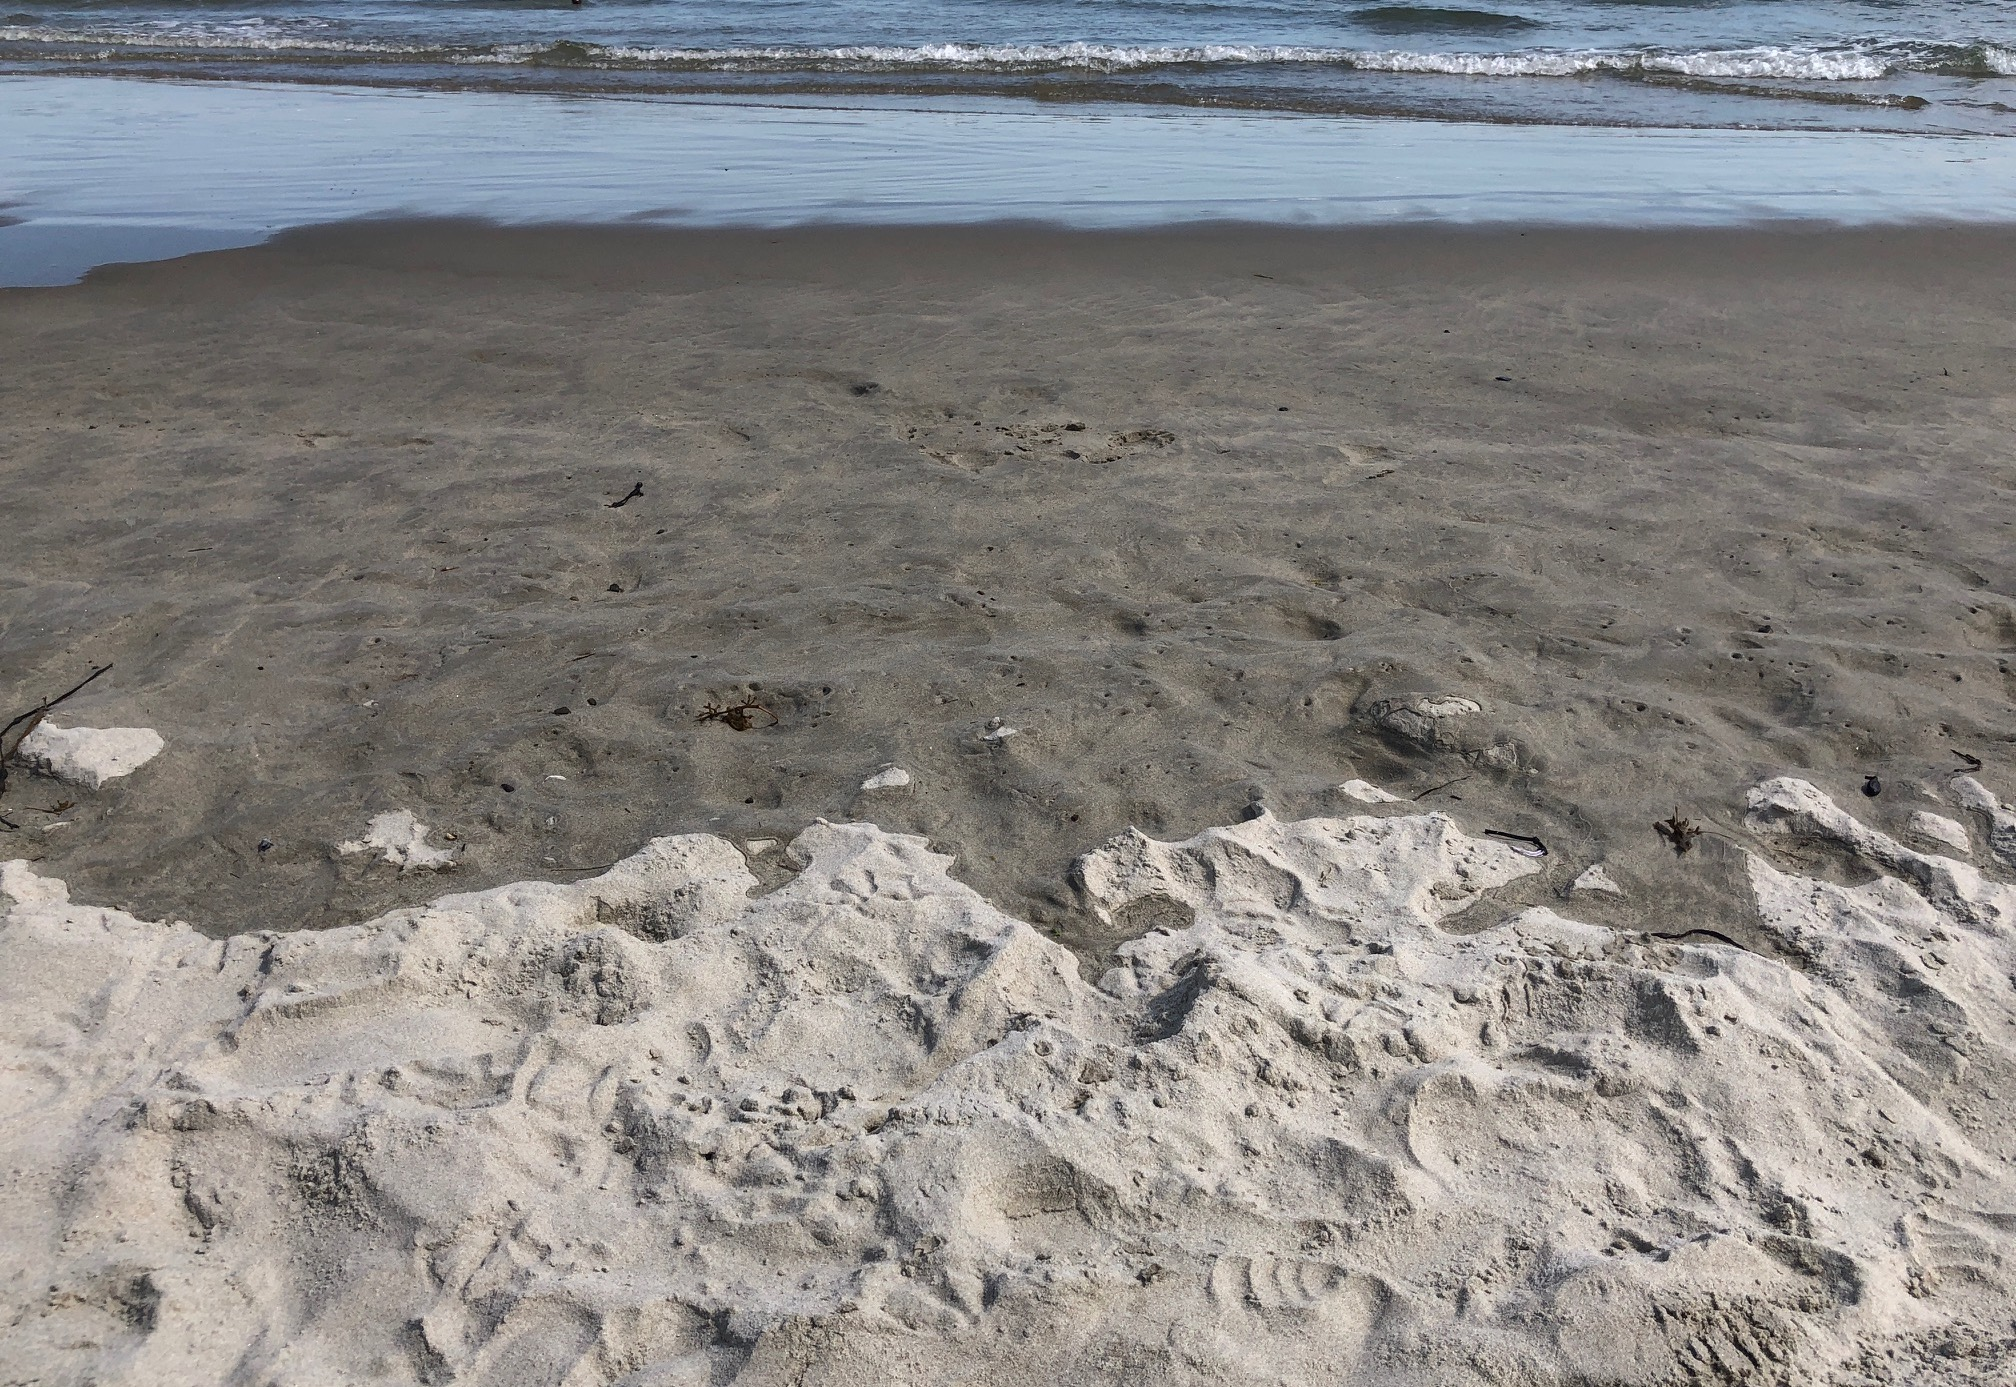
\includegraphics[width=.8\linewidth]{figures/visionscience/wet_sand_2.jpeg}}
    \caption{Why does wet sand look dark? The answer to this question is interesting, but not as much as the question itself.}
    \label{fig:wet_sand}
\end{figure}
% Photo by Antonio Torralba


Why does sand look darker when it's wet? Does everything wet look darker than when it is dry? How can we tell which parts of the sand are dark because they are wet and which ones are dark because they are under a shadow? 


\section{Concluding Remarks}

This chapter was about learning to ask questions about what we see, why things look the way they do, and how do we recognize them. There are so many things that we see every day that we recognize by the way they look, and yet we seldom ask ourselves why they look that way. Why does the sky appear blue? Why does the moon always look the same? Why do hot things become redder? 
There are many other sources you can consult that explore why things look the way they do in the world. A beautiful book on this topic is \booktitle{Light and Color in the Outdoors} by Marcel Minnaert \cite{Minnaert1993}, first published in 1937. 

After reading this chapter, you will not know how to implement anything new, nor will you have learned new math or new algorithms. The goal of this chapter was to show you some of the questions you should ask about the visual world that you experience every day. The exercise to do now is to go around with your camera and take pictures of interesting visual phenomena.

\marginnote{Your brain is like a detective looking at all the clues that reveal what the world is made of.} 
